%%-----------------------------------------------------------------------

\documentclass{styles/ufpethesis}
% Paquetes LaTeX y estilos globales

%\input{etc/style}
%%%%%%%%%%%%%%%%%%%%%%%%%%%%%%%%%%%%%%%%%%%%%%%%%%%%%%%%%%%%%%%%%%%%%%%%%
%%% ufpehesis.cls
%%% UFPE Thesis/Dissertation document class
%%% (C) 2003- Paulo Gustavo Soares Fonseca
%%% THIS FILE COMES WITH NO WARRANTIES
%%% PERMISSION TO COPY AND REDISTRIBUTE FREE OF CHARGE
%%% FOR ACADEMIC PURPOSES ONLY
%%%%%%%%%%%%%%%%%%%%%%%%%%%%%%%%%%%%%%%%%%%%%%%%%%%%%%%%%%%%%%%%%%%%%%%%
%%%    Author              = "Paulo G. S. Fonseca",
%%%    Version             = "1.0",
%%%    Date                = "Jul 2018",
%%%    Filename            = "ufpethesis.cls",
%%%    Address             = "Universidade Federal de Pernambuco
%%%                           Centro de Informática",
%%%    Telephone           = "+55 81 2126-8430",
%%%    Email               = "paguso@cin.ufpe.br",
%%%    Keywords            = "LaTeX, Thesis, Dissertation",
%%%    Abstract            = "LaTeX document-style for typesetting of
%%%                           Monographs, Theses and Dissertations at the
%%%                           Federal University of Pernambuco - Brazil"
%%%    SeeAlso             = "book.sty",
%%%%%%%%%%%%%%%%%%%%%%%%%%%%%%%%%%%%%%%%%%%%%%%%%%%%%%%%%%%%%%%%%%%%%%%%

\ProvidesClass{styles/ufpethesis}[2006/29/01]
%\input{styles/aboutufpethesis.txt}

%%%%%%%%%%%%%%%%%%%%%%%%%%%%%%%%%%%%%%%%%%%%%%%%%%%%%%%%%%%%%%%%%%%%%%%%
%% OPTIONS 
%%%%%%%%%%%%%%%%%%%%%%%%%%%%%%%%%%%%%%%%%%%%%%%%%%%%%%%%%%%%%%%%%%%%%%%%

\DeclareOption{pt}{%
  \let\@language=0%
  \PassOptionsToPackage{brazil}{babel}}

\DeclareOption{en}{%
  \let\@language=1%
  \PassOptionsToPackage{brazil,english}{babel}}

\DeclareOption{oneside}{%
  \PassOptionsToClass{oneside}{book}}

\DeclareOption{twoside}{%
  \PassOptionsToClass{twoside}{book}}
 
\DeclareOption{print}{%
  \let\@scr=0}

\DeclareOption{scr}{%
  \let\@scr=1%
  \PassOptionsToClass{dvipdfm}{book}}
  
\DeclareOption{bsc}{%
  \let\@degreetype=0}

\DeclareOption{msc}{%
  \let\@degreetype=1}

\DeclareOption{qual}{%
  \let\@degreetype=2}

\DeclareOption{prop}{%
  \let\@degreetype=3}

\DeclareOption{phd}{%
  \let\@degreetype=4}
  
\DeclareOption{classic}{%
  \let\@style=0}
 
\DeclareOption{modern}{%
  \let\@style=1
}

\DeclareOption{ugly}{%
  \let\@style=2
}

% Default options
\ExecuteOptions{en,phd,modern,print,twoside}
\ProcessOptions

\LoadClass[12pt,a4paper]{book}


%%%%%%%%%%%%%%%%%%%%%%%%%%%%%%%%%%%%%%%%%%%%%%%%%%%%%%%%%%%%%%%%%%%%%%%%
%% PACKAGES
%%%%%%%%%%%%%%%%%%%%%%%%%%%%%%%%%%%%%%%%%%%%%%%%%%%%%%%%%%%%%%%%%%%%%%%%
\RequirePackage{amsmath,amssymb,amsthm}%amsfonts,
\RequirePackage{babel}
\RequirePackage{calc}
\RequirePackage{ifthen}
\RequirePackage[utf8]{inputenc}
\RequirePackage{textcase}
\RequirePackage{textcomp}
\RequirePackage{url}
\RequirePackage{xspace}
\if\@style1
%\usepackage[utf8]{inputenc}
  \RequirePackage[T1]{fontenc}
%\RequirePackage[utf8]{inputenc}
  %\RequirePackage{mathptmx}
  \RequirePackage[scaled=0.92]{helvet}
  \RequirePackage{courier}
\fi
\if\@scr0
  \RequirePackage{graphicx}
\fi
\if\@scr1
  \RequirePackage{graphicx}
  \RequirePackage[usenames]{color}
  \RequirePackage[colorlinks,backref]{hyperref}
\fi


%%%%%%%%%%%%%%%%%%%%%%%%%%%%%%%%%%%%%%%%%%%%%%%%%%%%%%%%%%%%%%%%%%%%%%%%
%% GENERAL PURPOSE MACROS
%%%%%%%%%%%%%%%%%%%%%%%%%%%%%%%%%%%%%%%%%%%%%%%%%%%%%%%%%%%%%%%%%%%%%%%%
\let\origcleardoublepage=\cleardoublepage
\def\cleardoublepage{%
 % \newpage{\pagestyle{empty}\origcleardoublepage}
}

%%
% For use with the pseudocode package
\def\@lopcchapterspace{\relax}

%%%%%%%%%%%%%%%%%%%%%%%%%%%%%%%%%%%%%%%%%%%%%%%%%%%%%%%%%%%%%%%%%%%%%%%%
%% LABELS
%%%%%%%%%%%%%%%%%%%%%%%%%%%%%%%%%%%%%%%%%%%%%%%%%%%%%%%%%%%%%%%%%%%%%%%%

%% Language Independent

\gdef\@maleadvisertitle{Orientador}
\gdef\@femaleadvisertitle{Orientadora}
\gdef\@malecoadvisertitle{Co-orientador}
\gdef\@femalecoadvisertitle{Co-orientadora}
\gdef\@bachelordissertation{Trabalho de Graduação}
\gdef\@mastersdissertation{Dissertação de Mestrado}
\gdef\@phdqualifying{Monografia de Qualificação}
\gdef\@phdproposal{Proposta de Tese de Doutorado}
\gdef\@phdthesis{Tese de Doutorado}
\gdef\@bachelordegree{Bacharel}
\gdef\@mastersdegree{Mestre}
\gdef\@phddegree{Doutora}
\gdef\@presentationtext{%
Trabalho apresentado ao Programa de
\@program\ do \if\@showdepartment1\@department\ \else\@institute\ \fi
da \@university\ como requisito para obtenção do
grau de \@phddegree\ em \@majorfield.}
\gdef\resumoname{Resumo}
\gdef\abstrname{Abstract}
\gdef\keywordsnamePT{Palavras-chave}
\gdef\keywordsnameEN{Keywords}

%% Language Dependent

% Portuguese
\if\@language0
  \gdef\@notdefined{Estatística}
  \gdef\acknowledgementsname{Agradecimentos}
  \gdef\@axiomname{Axioma}
  \gdef\@conjecturename{Conjectura}
  \gdef\@defname{Definição}
  \gdef\@lemmaname{Lema}
  \gdef\@theoname{Teorema}
  \gdef\@propname{Proposição}
  \gdef\@corname{Corolário}
  \gdef\@proofname{Prova}
  \gdef\@examplename{Exemplo}
  \gdef\@figurename{Figura}
  \gdef\@tablename{Tabela}
  \gdef\@equationame{equação}
  \gdef\@chaptername{Capítulo}
  \gdef\@sectionname{Seção}
  \gdef\@appendixname{Apêndice}
  \gdef\@pagename{página}
  \gdef\@colophontext{%
  \urlstyle{rm}%
  Este volume foi tipografado em \LaTeX\ na classe \textsf{UFPEThesis}
  (\url{www.cin.ufpe.br/~paguso/ufpethesis}).
  \if\@scr1
  Para detalhes sobre este documento, clique \Acrobatmenu{GeneralInfo}{aqui}.
  \fi}
% English
\else\if\@language1
  \gdef\@notdefined{Estatística}
  \gdef\acknowledgementsname{Acknowledgements}
  \gdef\@axiomname{Axiom}
  \gdef\@conjecturename{Conjecture}
  \gdef\@defname{Definition}
  \gdef\@lemmaname{Lemma}
  \gdef\@theoname{Theorem}
  \gdef\@propname{Proposition}
  \gdef\@corname{Corollary}
  \gdef\@proofname{Proof}
  \gdef\@examplename{Example}
  \gdef\@figurename{Figure}
  \gdef\@tablename{Table}
  \gdef\@equationame{equation}
  \gdef\@chaptername{Chapter}
  \gdef\@sectionname{Section}
  \gdef\@appendixname{Appendix}
  \gdef\@pagename{page}
  \gdef\@colophontext{%
  \urlstyle{rm}%
  This volume has been typeset in \LaTeX with the \textsf{UFPEThesis} class
  (\url{www.cin.ufpe.br/~paguso/ufpethesis}).
  \if\@scr1
  For details about this document, click \Acrobatmenu{GeneralInfo}{here}. 
  \fi}
\fi\fi


%%%%%%%%%%%%%%%%%%%%%%%%%%%%%%%%%%%%%%%%%%%%%%%%%%%%%%%%%%%%%%%%%%%%%%%%
%% IDENTIFICATION
%%%%%%%%%%%%%%%%%%%%%%%%%%%%%%%%%%%%%%%%%%%%%%%%%%%%%%%%%%%%%%%%%%%%%%%%

%% School identification

\def\university#1{%
  \gdef\@university{#1}}
\def\@university{Universidade Federal de Pernambuco}

\def\universitylogo{
\includegraphics{styles/logos/ufpelogo.pdf}}

\let\@showinstitute=0
\def\institute#1{%
  \let\@showinstitute=1
  \gdef\@institute{#1}}

\let\@showdepartment=0
\def\department#1{%
  \let\@showdepartment=1
  \gdef\@department{#1}}

\def\program#1{%
  \gdef\@program{#1}}
\def\@program{\@notdefined}

\def\majorfield#1{%
  \gdef\@majorfield{#1}}
\def\@majorfield{\@notdefined}

\def\address#1{%
  \gdef\@address{#1}}
\def\@address{Recife}

%% Authors identification

\def\author#1{%
  \gdef\@author{#1}
  \if\@scr1 \hypersetup{pdfauthor={\@author}}\fi}
\def\@author{\@notdefined}

\def\adviser{%
  \@ifnextchar [%
    {\@padviser}%
    {\@padviser[\@empty]}}
\def\@padviser[#1]#2{%
  \ifx#1\@empty
    \gdef\@advisertitle{\@maleadvisertitle}
  \else
    \gdef\@advisertitle{\@femaleadvisertitle}
  \fi
  \gdef\@adviser{#2}}
\def\@adviser{\@notdefined}

\let\@showcoadviser=0
\def\coadviser{%
  \@ifnextchar [%
    {\@pcoadviser}%
    {\@pcoadviser[\@empty]}}
\def\@pcoadviser[#1]#2{%
  \let\@showcoadviser=1
  \ifx#1\@empty
    \gdef\@coadvisertitle{\@malecoadvisertitle}
  \else
    \gdef\@coadvisertitle{\@femalecoadvisertitle}
  \fi
  \gdef\@coadviser{#2}}

%% Work identification

\def\title#1{%
  \gdef\@title{#1}
  \if\@scr1 \hypersetup{pdftitle={\@title}}\fi}
\def\@title{\@notdefined}

\def\@texttype{%
  \if\@degreetype0
    \@bachelordissertation
  \else\if\@degreetype1
    \@mastersdissertation
  \else\if\@degreetype2
    \@phdqualifying
  \else\if\@degreetype3
    \@phdproposal
  \else\if\@degreetype4
    \@phdthesis
  \fi\fi\fi\fi\fi}

\def\@degree{%
  \if\@degreetype0
    \@bachelordegree
  \else\if\@degreetype1
    \@mastersdegree
  \else\if\@degreetype2
    \@phddegree
  \else\if\@degreetype3
    \@phddegree
  \else\if\@degreetype4
    \@phddegree
  \fi\fi\fi\fi\fi}


%%%%%%%%%%%%%%%%%%%%%%%%%%%%%%%%%%%%%%%%%%%%%%%%%%%%%%%%%%%%%%%%%%%%%%%%
%% PAGE LAYOUT
%%%%%%%%%%%%%%%%%%%%%%%%%%%%%%%%%%%%%%%%%%%%%%%%%%%%%%%%%%%%%%%%%%%%%%%%

\setlength{\topmargin}{0mm}
\setlength{\textheight}{\paperheight-\headheight-\headsep-\footskip-2in}
\setlength{\oddsidemargin}{0mm}
\setlength{\evensidemargin}{0mm}
\setlength{\marginparwidth}{0mm}
\setlength{\marginparsep}{0mm}
\setlength{\textwidth}{\paperwidth-2in}


%%%%%%%%%%%%%%%%%%%%%%%%%%%%%%%%%%%%%%%%%%%%%%%%%%%%%%%%%%%%%%%%%%%%%%%%
%%%%%%%%%%%%%%%%%%%         CLASSIC STYLE            %%%%%%%%%%%%%%%%%%%
%%%%%%%%%%%%%%%%%%%%%%%%%%%%%%%%%%%%%%%%%%%%%%%%%%%%%%%%%%%%%%%%%%%%%%%%
\if\@style0


%%%%%%%%%%%%%%%%%%%%%%%%%%%%%%%%%%%%%%%%%%%%%%%%%%%%%%%%%%%%%%%%%%%%%%%%
%% Fonts
%%%%%%%%%%%%%%%%%%%%%%%%%%%%%%%%%%%%%%%%%%%%%%%%%%%%%%%%%%%%%%%%%%%%%%%%

\font\quotefont=cmssq8 scaled\magstep1
\font\quotefonti=cmssqi8 scaled\magstep1


%%%%%%%%%%%%%%%%%%%%%%%%%%%%%%%%%%%%%%%%%%%%%%%%%%%%%%%%%%%%%%%%%%%%%%%%
%% Frontpage
%%%%%%%%%%%%%%%%%%%%%%%%%%%%%%%%%%%%%%%%%%%%%%%%%%%%%%%%%%%%%%%%%%%%%%%%

\def\frontpage{%
	\if@openright\cleardoublepage\else\clearpage\fi
  \thispagestyle{empty}
  \begin{center}
  \universitylogo
  \sf\large
  \\\@university
  \if\@showinstitute1\\\@institute\fi
  \if\@showdepartment1\\\@department\fi
  \vskip 25mm
  \@program
  \vskip 45mm
  \begin{minipage}{110mm}
    \begin{center}
      \textbf{\MakeTextUppercase{\@title}}
      \vskip\baselineskip
      \@author
      \vskip\baselineskip
      \MakeTextUppercase{\@texttype}
    \end{center}
  \end{minipage}\\
  \vfill
  \@address\\
  \@date
  \end{center}
}


%%%%%%%%%%%%%%%%%%%%%%%%%%%%%%%%%%%%%%%%%%%%%%%%%%%%%%%%%%%%%%%%%%%%%%%%
%% Presentation page
%%%%%%%%%%%%%%%%%%%%%%%%%%%%%%%%%%%%%%%%%%%%%%%%%%%%%%%%%%%%%%%%%%%%%%%%

\def\presentationpage{%
  \if@openright\cleardoublepage\else\clearpage\fi
  \thispagestyle{empty}
	~\\
  \begin{center}
  \sf\large
  \@university
  \if\@showinstitute1\\\@institute\fi
  \if\@showdepartment1\\\@department\fi
  \vskip 25mm
  \@author
  \vskip\baselineskip
  \textbf{\MakeTextUppercase{\@title}}
  \vskip 58mm
  \begin{flushright}
    \begin{minipage}{100mm}
    \quotefonti %
    \@presentationtext
    \vskip2\baselineskip
    {\quotefont \@advisertitle:} \@adviser
    \if\@showcoadviser1
      \\ {\quotefont\@coadvisertitle:} \@coadviser
    \fi
    \end{minipage}
  \end{flushright}
  \vfill
  \@address\\
  \@date
  \end{center}
}


%%%%%%%%%%%%%%%%%%%%%%%%%%%%%%%%%%%%%%%%%%%%%%%%%%%%%%%%%%%%%%%%%%%%%%%%
%% Dedicatory
%%%%%%%%%%%%%%%%%%%%%%%%%%%%%%%%%%%%%%%%%%%%%%%%%%%%%%%%%%%%%%%%%%%%%%%%

\def\dedicatory{%
  \if@openright\cleardoublepage\else\clearpage\fi
  \thispagestyle{empty}
  ~\\
  \vfill
  \begin{flushright}
    \begin{minipage}{100mm}
    \quotefonti}
\def\enddedicatory{
    \normalfont
    \end{minipage}
  \end{flushright}}


%%%%%%%%%%%%%%%%%%%%%%%%%%%%%%%%%%%%%%%%%%%%%%%%%%%%%%%%%%%%%%%%%%%%%%%%
%% Acknowledgements
%%%%%%%%%%%%%%%%%%%%%%%%%%%%%%%%%%%%%%%%%%%%%%%%%%%%%%%%%%%%%%%%%%%%%%%%

\def\acknowledgements{%
  \chapter*{\acknowledgementsname}}


%%%%%%%%%%%%%%%%%%%%%%%%%%%%%%%%%%%%%%%%%%%%%%%%%%%%%%%%%%%%%%%%%%%%%%%%
%% Resumo
%%%%%%%%%%%%%%%%%%%%%%%%%%%%%%%%%%%%%%%%%%%%%%%%%%%%%%%%%%%%%%%%%%%%%%%%

\def\resumo{%
  \gdef\@keywordsname{\keywordsnamePT}
  \chapter*{\resumoname}}


%%%%%%%%%%%%%%%%%%%%%%%%%%%%%%%%%%%%%%%%%%%%%%%%%%%%%%%%%%%%%%%%%%%%%%%%
%% Abstract
%%%%%%%%%%%%%%%%%%%%%%%%%%%%%%%%%%%%%%%%%%%%%%%%%%%%%%%%%%%%%%%%%%%%%%%%

\def\abstract{%
  \gdef\@keywordsname{\keywordsnameEN}
  \chapter*{\abstrname}}

  
%%%%%%%%%%%%%%%%%%%%%%%%%%%%%%%%%%%%%%%%%%%%%%%%%%%%%%%%%%%%%%%%%%%%%%%%
%% Keywords
%%%%%%%%%%%%%%%%%%%%%%%%%%%%%%%%%%%%%%%%%%%%%%%%%%%%%%%%%%%%%%%%%%%%%%%%

\def\@keywordsname{\@defaultkeywordsname}
\def\keywords{%
  \par\vskip\baselineskip\noindent{\bf\@keywordsname: }}
\def\endkeywords{}


%%%%%%%%%%%%%%%%%%%%%%%%%%%%%%%%%%%%%%%%%%%%%%%%%%%%%%%%%%%%%%%%%%%%%%%%
%% Quotations
%%%%%%%%%%%%%%%%%%%%%%%%%%%%%%%%%%%%%%%%%%%%%%%%%%%%%%%%%%%%%%%%%%%%%%%%

\def\epigraph{%
  \if@openright\cleardoublepage\else\clearpage\fi
  \thispagestyle{empty}
  ~\\\vfill
  \begin{quotation}}
\def\endepigraph{\end{quotation}}

\def\quotation{%
  \@ifnextchar [%
    {\begin{pquot@tion}}%
    {\begin{pquot@tion}[\@empty]}}
\def\endquotation{\end{pquot@tion}\@afterindentfalse}

\def\pquot@tion[#1]#2{%
  \gdef\@qauthor{#2}
  \gdef\@qnote{#1}
  \begin{flushright}
    \begin{minipage}{0.8\textwidth}
      \begin{flushright}\quotefonti}
\def\endpquot@tion{%
        \vskip.2\baselineskip%
        \quotefont---\MakeTextUppercase{\@qauthor}
        \if\@qnote\@empty
          \relax
        \else
          \space(\@qnote)
        \fi
      \end{flushright}
    \end{minipage}
  \end{flushright}
  \normalfont\vskip\baselineskip}

  
%%%%%%%%%%%%%%%%%%%%%%%%%%%%%%%%%%%%%%%%%%%%%%%%%%%%%%%%%%%%%%%%%%%%%%%%
%% Table of contents
%%%%%%%%%%%%%%%%%%%%%%%%%%%%%%%%%%%%%%%%%%%%%%%%%%%%%%%%%%%%%%%%%%%%%%%%

\renewcommand\tableofcontents{%
  \chapter*{\contentsname}
  \@starttoc{toc}}

\def\l@part#1#2{%
  \ifnum \c@tocdepth >-2\relax
    \addpenalty{-\@highpenalty}%
    \addvspace{2.25em \@plus\p@}%
    \setlength\@tempdima{3em}%
    \begingroup
      \parindent \z@ \rightskip \@pnumwidth
      \parfillskip -\@pnumwidth
      {\leavevmode
       \large\sf\bfseries #1\hfil \hb@xt@\@pnumwidth{\hss}}\par
       \nobreak
         \global\@nobreaktrue
         \everypar{\global\@nobreakfalse\everypar{}}%
    \endgroup
  \fi}
\def\l@chapter#1#2{%
  \ifnum \c@tocdepth >\m@ne
    \addpenalty{-\@highpenalty}%
    \vskip 1.0em \@plus\p@
    \setlength\@tempdima{1.5em}%
    \begingroup
      \parindent \z@ \rightskip \@pnumwidth
      \parfillskip -\@pnumwidth
      \leavevmode %\sffamily\bfseries
      \advance\leftskip\@tempdima
      \hskip -\leftskip
      %\vskip .1\baselineskip
	  {\sffamily\bfseries #1}\nobreak\hfil \nobreak\hb@xt@\@pnumwidth{\hss #2}\par
	  \vskip .6\baselineskip
      \penalty\@highpenalty
    \endgroup
  \fi}

\setcounter{tocdepth}{4}


%%%%%%%%%%%%%%%%%%%%%%%%%%%%%%%%%%%%%%%%%%%%%%%%%%%%%%%%%%%%%%%%%%%%%%%%
%% Sectioning
%%%%%%%%%%%%%%%%%%%%%%%%%%%%%%%%%%%%%%%%%%%%%%%%%%%%%%%%%%%%%%%%%%%%%%%%

\setcounter{secnumdepth}{4}

\def\part{%
  \if@openright\cleardoublepage\else\clearpage\fi
  \thispagestyle{empty}%
  \secdef\@part\@spart}
\def\@part[#1]#2{%
    \ifnum \c@secnumdepth >-2\relax
      \refstepcounter{part}%
      \addcontentsline{toc}{part}{\thepart\hspace{1em}#1}%
    \else
      \addcontentsline{toc}{part}{#1}%
    \fi
    \markboth{}{}%
    {\centering
     \interlinepenalty \@M
     \normalfont
     \null\vfil
     \ifnum \c@secnumdepth >-2\relax
       \Large\sf \MakeTextUppercase{\partname\nobreakspace\thepart}
       \par
       \vskip 20\p@
     \fi
     \huge\bfseries\MakeTextUppercase{#2}\par}
     \vfil}
\def\@spart#1{%
    {\centering
     \interlinepenalty \@M
     \normalfont
     \null\vfil
     \huge\sf\bfseries\MakeTextUppercase{#1}\par}
     \vfil}

\def\chapter{\if@openright\cleardoublepage\else\clearpage\fi
             \thispagestyle{plain}%
             \global\@topnum\z@
             \@afterindentfalse
             \secdef\@chapter\@schapter}

\def\@chapter[#1]#2{
   \refstepcounter{chapter}%
   \addcontentsline{toc}{chapter}{\chaptername~\thechapter---#1}%
   \chaptermark{#1}%
   \addtocontents{lof}{\protect\addvspace{10\p@}}%
   \addtocontents{lot}{\protect\addvspace{10\p@}}%
   \@lopcchapterspace%
   \@makechapterhead{#2}%
   \@afterheading}

\def\@makechapterhead#1{%
  {\noindent\sffamily\large\MakeTextUppercase{\chaptername~\thechapter}}%
  \vskip 2\baselineskip%
  {\begin{flushright}\Large\sffamily\bfseries\MakeTextUppercase{#1}\end{flushright}}%
  \vskip 1.5\baselineskip}

\def\@schapter#1{%
  \chaptermark{#1}%
  \@makeschapterhead{#1}%
  \@afterheading}

\def\@makeschapterhead#1{%
  {\noindent\sffamily\large\MakeTextUppercase{~}}%
  \vskip 2\baselineskip%
  {\begin{flushright}\Large\sffamily\bfseries\MakeTextUppercase{#1}\end{flushright}}
  \vskip 1.5\baselineskip}

\def\appendix{%
   \setcounter{chapter}{0}%
   \renewcommand{\thechapter}{\Alph{chapter}}%
   \renewcommand{\chaptername}{\appendixname}
	 \renewcommand{\theequation}{\thechapter.\oldstylenums{\arabic{equation}}}
}

\def\@startsection#1#2#3#4#5#6{%
 \if@noskipsec \leavevmode \fi
 \par \@tempskipa #4\relax
 \@afterindentfalse
 \ifdim \@tempskipa <\z@ \@tempskipa -\@tempskipa \@afterindentfalse\fi
 \if@nobreak \everypar{}\else
     \addpenalty\@secpenalty\addvspace\@tempskipa\fi
 \@ifstar{\@dblarg{\@sect{#1}{\@m}{#3}{#4}{#5}{#6}}}%
         {\@dblarg{\@sect{#1}{#2}{#3}{#4}{#5}{#6}}}%
}

\def\section{%
  \@startsection{section}{1}{0mm}{\baselineskip}
    {.625\baselineskip}{\sffamily\bfseries\MakeTextUppercase}}

\def\subsection{%
  \@startsection{subsection}{2}{0mm}{\baselineskip}
    {.6\baselineskip}{\sffamily\bfseries}}

\def\subsubsection{%
  \@startsection{subsubsection}{3}{0mm}{1.2\baselineskip}
   {-1em}{\rm\bfseries}}

\def\paragraph{%
  \@startsection{paragraph}{4}{0mm}{\baselineskip}
   {-1em}{\itshape}}

\def\colophon{%
  \if@openright\cleardoublepage\else\clearpage\fi
  \thispagestyle{empty}
  \null\vfill
  \small\noindent\@colophontext
}


%%%%%%%%%%%%%%%%%%%%%%%%%%%%%%%%%%%%%%%%%%%%%%%%%%%%%%%%%%%%%%%%%%%%%%%%
%% Headers & footers
%%%%%%%%%%%%%%%%%%%%%%%%%%%%%%%%%%%%%%%%%%%%%%%%%%%%%%%%%%%%%%%%%%%%%%%%
\def\chaptermark#1%
{\markboth{\normalfont\footnotesize\MakeTextUppercase{#1}}%
{\normalfont\scriptsize\MakeTextUppercase{#1}}}

\def\schaptermark#1%
{\markboth{\normalfont\footnotesize\MakeTextUppercase{#1}}%
{\normalfont\scriptsize\MakeTextUppercase{#1}}}

\def\sectionmark#1%
{\markright{\normalfont\footnotesize\MakeTextUppercase{\thesection\ #1}}}

%\def\chaptermark#1{\markboth{\sc\MakeLowercase{#1}}{\sc\MakeLowercase{#1}}}
%\def\sectionmark#1{\markright{\sc\MakeLowercase{\thesection\ #1}}}

%%%%%%%%%%%%%%%%%%%%%%%%%%%%%%%%%%%%%%%%%%%%%%%%%%%%%%%%%%%%%%%%%%%%%%%%
%% Bibliography
%%%%%%%%%%%%%%%%%%%%%%%%%%%%%%%%%%%%%%%%%%%%%%%%%%%%%%%%%%%%%%%%%%%%%%%%

\global\renewenvironment{thebibliography}[1]
     {\chapter*{\bibname}%
      \list{\@biblabel{\@arabic\c@enumiv}}%
           {\settowidth\labelwidth{\@biblabel{#1}}%
            \leftmargin\labelwidth
            \advance\leftmargin\labelsep
            \@openbib@code
            \usecounter{enumiv}%
            \let\p@enumiv\@empty
            \renewcommand\theenumiv{\@arabic\c@enumiv}}%
      \sloppy
      \clubpenalty4000
      \@clubpenalty \clubpenalty
      \widowpenalty4000%
      \sfcode`\.\@m}
     {\def\@noitemerr
       {\@latex@warning{Empty `thebibliography' environment}}%
      \endlist}


%%%%%%%%%%%%%%%%%%%%%%%%%%%%%%%%%%%%%%%%%%%%%%%%%%%%%%%%%%%%%%%%%%%%%%%%
%% Tables and figures
%%%%%%%%%%%%%%%%%%%%%%%%%%%%%%%%%%%%%%%%%%%%%%%%%%%%%%%%%%%%%%%%%%%%%%%%

\long\def\@makecaption#1#2{%
  \vskip\abovecaptionskip
  \sbox\@tempboxa{\small\bf #1\rm\enskip #2}%
  \ifdim \wd\@tempboxa >\hsize
    {\small\bf#1\rm\enskip #2\par}
  \else
    \global \@minipagefalse
    \hb@xt@\hsize{\hfil\box\@tempboxa\hfil}%
  \fi
  \vskip\belowcaptionskip}


%%%%%%%%%%%%%%%%%%%%%%%%%%%%%%%%%%%%%%%%%%%%%%%%%%%%%%%%%%%%%%%%%%%%%%%%
%% Mathematics
%%%%%%%%%%%%%%%%%%%%%%%%%%%%%%%%%%%%%%%%%%%%%%%%%%%%%%%%%%%%%%%%%%%%%%%%

% Equation numbering
\renewcommand{\theequation}{\oldstylenums{\thechapter}.\oldstylenums{\arabic{equation}}}

% Theorem-like environments
\newtheoremstyle{theo}%
	{\topsep}{\topsep}% Space above and below
	{\slshape}% Body style
	{0pt}% Heading indent amount
	{\bfseries}{.}% Heading font and punctuation after it
	{1ex plus 0pt minus .2ex}% Space after heading 
	{}% Head spec (empty = same as ‘plain’ style
\theoremstyle{definition}
\newtheorem{Def}{\@defname}[chapter]
\newtheorem{Exp}{\@examplename}[chapter]
\theoremstyle{theo}
\newtheorem{Axi}{\@axiomname}[chapter]
\newtheorem{Conj}{\@conjecturename}[chapter]
\newtheorem{Lem}{\@lemmaname}[chapter]
\newtheorem{Theo}{\@theoname}[chapter]
\newtheorem{Prop}{\@propname}[chapter]
\newtheorem{Cor}{\@corname}[chapter]
\renewcommand{\qedsymbol}{\rule{3pt}{8pt}}


%%%%%%%%%%%%%%%%%%%%%%%%%%%%%%%%%%%%%%%%%%%%%%%%%%%%%%%%%%%%%%%%%%%%%%%%
% Reference macros
%%%%%%%%%%%%%%%%%%%%%%%%%%%%%%%%%%%%%%%%%%%%%%%%%%%%%%%%%%%%%%%%%%%%%%%%

\newcommand{\figref}[2][]{\@figurename~\ref{#2}#1\xspace}
\newcommand{\tabref}[1]{\@tablename~\ref{#1}\xspace}
\newcommand{\eqnref}[1]{\@equationame~\eqref{#1}\xspace}
\newcommand{\chapref}[1]{\@chaptername~\ref{#1}\xspace}
\newcommand{\secref}[1]{\@sectionname~\ref{#1}\xspace}
\newcommand{\appref}[1]{\@appendixname~\ref{#1}\xspace}
\newcommand{\axiref}[1]{\@axiomname~\ref{#1}\xspace}
\newcommand{\conjref}[1]{\@conjname~\ref{#1}\xspace}
\newcommand{\defref}[1]{\@defname~\ref{#1}\xspace}
\newcommand{\lemref}[1]{\@lemmaname~\ref{#1}\xspace}
\newcommand{\theoref}[1]{\@theoname~\ref{#1}\xspace}
\newcommand{\corref}[1]{\@corname~\ref{#1}\xspace}
\newcommand{\propref}[1]{\@propname~\ref{#1}\xspace}
\newcommand{\expref}[1]{\@examplename~\ref{#1}\xspace}
\newcommand{\pgref}[1]{\@pagename~\pageref{#1}\xspace}



%%%%%%%%%%%%%%%%%%%%%%%%%%%%%%%%%%%%%%%%%%%%%%%%%%%%%%%%%%%%%%%%%%%%%%%%
%%%%%%%%%%%%%%%%%%%         STANDARD STYLE           %%%%%%%%%%%%%%%%%%%
%%%%%%%%%%%%%%%%%%%%%%%%%%%%%%%%%%%%%%%%%%%%%%%%%%%%%%%%%%%%%%%%%%%%%%%%
\else\if\@style1


%%%%%%%%%%%%%%%%%%%%%%%%%%%%%%%%%%%%%%%%%%%%%%%%%%%%%%%%%%%%%%%%%%%%%%%%
%% Fonts
%%%%%%%%%%%%%%%%%%%%%%%%%%%%%%%%%%%%%%%%%%%%%%%%%%%%%%%%%%%%%%%%%%%%%%%%

\newcommand\quotefont{\normalfont\normalsize}
\newcommand\quotefonti{\it\normalsize}


%%%%%%%%%%%%%%%%%%%%%%%%%%%%%%%%%%%%%%%%%%%%%%%%%%%%%%%%%%%%%%%%%%%%%%%%
%% Frontpage
%%%%%%%%%%%%%%%%%%%%%%%%%%%%%%%%%%%%%%%%%%%%%%%%%%%%%%%%%%%%%%%%%%%%%%%%

\def\frontpage{%
  \if@openright\cleardoublepage\else\clearpage\fi
  \thispagestyle{empty}
  \begin{center}
  \universitylogo
  \large
  \\\@university
  \if\@showinstitute1\\\@institute\fi
  \if\@showdepartment1\\\@department\fi
  \vskip 25mm
  \@program
  \vskip 45mm
  \begin{minipage}{110mm}
    \begin{center}
      {\Large\bfseries\@title}
      \vskip\baselineskip
      \@author
      \vskip\baselineskip
      \@texttype
    \end{center}
  \end{minipage}\\
  \vfill
  \@address\\
  \@date
  \end{center}
}


%%%%%%%%%%%%%%%%%%%%%%%%%%%%%%%%%%%%%%%%%%%%%%%%%%%%%%%%%%%%%%%%%%%%%%%%
%% Presentation page
%%%%%%%%%%%%%%%%%%%%%%%%%%%%%%%%%%%%%%%%%%%%%%%%%%%%%%%%%%%%%%%%%%%%%%%%

\def\presentationpage{%
  \if@openright\cleardoublepage\else\clearpage\fi
  \thispagestyle{empty}
		~\\
  \begin{center}
  \large
  \@university
  \if\@showinstitute1\\\@institute\fi
  \if\@showdepartment1\\\@department\fi
  \vskip 25mm
  \@author
  \vskip\baselineskip
  {\Large\bfseries\@title}
  \vskip 58mm
  %\begin{flushright}
    \begin{minipage}{100mm}
    \quotefonti %
    \@presentationtext
    \vskip2\baselineskip
    \begin{center}
    \begin{tabular}{rl}
    {\quotefont \@advisertitle:}&\@adviser\\
    \if\@showcoadviser1{\quotefont\@coadvisertitle:}&\@coadviser\\\fi
    \end{tabular}
    \end{center}
    \end{minipage}
  %\end{flushright}
  \vfill \vfill \vfill \vfill
  \@address\\ 
  \@date
  \end{center}
}


%%%%%%%%%%%%%%%%%%%%%%%%%%%%%%%%%%%%%%%%%%%%%%%%%%%%%%%%%%%%%%%%%%%%%%%%
%% Dedicatory
%%%%%%%%%%%%%%%%%%%%%%%%%%%%%%%%%%%%%%%%%%%%%%%%%%%%%%%%%%%%%%%%%%%%%%%%

\def\dedicatory{%
  \if@openright\cleardoublepage\else\clearpage\fi
  \thispagestyle{empty}
  ~\\
  \vfill
  \begin{flushright}
    \begin{minipage}{100mm}
    \quotefonti
    \begin{flushright}}
\def\enddedicatory{
		\end{flushright}
    \normalfont
    \end{minipage}
  \end{flushright}}


%%%%%%%%%%%%%%%%%%%%%%%%%%%%%%%%%%%%%%%%%%%%%%%%%%%%%%%%%%%%%%%%%%%%%%%%
%% Acknowledgements
%%%%%%%%%%%%%%%%%%%%%%%%%%%%%%%%%%%%%%%%%%%%%%%%%%%%%%%%%%%%%%%%%%%%%%%%

\def\acknowledgements{%
  \chapter*{\acknowledgementsname}}


%%%%%%%%%%%%%%%%%%%%%%%%%%%%%%%%%%%%%%%%%%%%%%%%%%%%%%%%%%%%%%%%%%%%%%%%
%% Resumo
%%%%%%%%%%%%%%%%%%%%%%%%%%%%%%%%%%%%%%%%%%%%%%%%%%%%%%%%%%%%%%%%%%%%%%%%

\def\resumo{%
  \gdef\@keywordsname{\keywordsnamePT}
  \chapter*{\resumoname}}


%%%%%%%%%%%%%%%%%%%%%%%%%%%%%%%%%%%%%%%%%%%%%%%%%%%%%%%%%%%%%%%%%%%%%%%%
%% Abstract
%%%%%%%%%%%%%%%%%%%%%%%%%%%%%%%%%%%%%%%%%%%%%%%%%%%%%%%%%%%%%%%%%%%%%%%%

\def\abstract{%
  \gdef\@keywordsname{\keywordsnameEN}
  \chapter*{\abstrname}}

  
%%%%%%%%%%%%%%%%%%%%%%%%%%%%%%%%%%%%%%%%%%%%%%%%%%%%%%%%%%%%%%%%%%%%%%%%
%% Keywords
%%%%%%%%%%%%%%%%%%%%%%%%%%%%%%%%%%%%%%%%%%%%%%%%%%%%%%%%%%%%%%%%%%%%%%%%

\def\@keywordsname{\@defaultkeywordsname}
\def\keywords{%
  \par\vskip\baselineskip\noindent{\bf\@keywordsname: }}
\def\endkeywords{}


%%%%%%%%%%%%%%%%%%%%%%%%%%%%%%%%%%%%%%%%%%%%%%%%%%%%%%%%%%%%%%%%%%%%%%%%
%% Quotations
%%%%%%%%%%%%%%%%%%%%%%%%%%%%%%%%%%%%%%%%%%%%%%%%%%%%%%%%%%%%%%%%%%%%%%%%

\def\epigraph{%
  \if@openright\cleardoublepage\else\clearpage\fi
  \thispagestyle{empty}
  ~\\\vfill
  \begin{quotation}}
\def\endepigraph{\end{quotation}}

\def\quotation{%
  \@ifnextchar [%
    {\begin{pquot@tion}}%
    {\begin{pquot@tion}[\@empty]}}
\def\endquotation{\end{pquot@tion}\@afterindentfalse\@afterheading}

\def\pquot@tion[#1]#2{%
  \def\@qauthor{#2}
  \def\@qnote{#1}
  \begin{flushright}
    \begin{minipage}{0.8\textwidth}
      \begin{flushright}\quotefonti}
\def\endpquot@tion{%
        \vskip.2\baselineskip%
        \quotefont---\MakeTextUppercase{\@qauthor}
        \if\@qnote\@empty
          \relax
        \else
          \space(\@qnote)
        \fi
      \end{flushright}
    \end{minipage}
  \end{flushright}
  \normalfont\vskip2\baselineskip}

  
%%%%%%%%%%%%%%%%%%%%%%%%%%%%%%%%%%%%%%%%%%%%%%%%%%%%%%%%%%%%%%%%%%%%%%%%
%% Table of contents
%%%%%%%%%%%%%%%%%%%%%%%%%%%%%%%%%%%%%%%%%%%%%%%%%%%%%%%%%%%%%%%%%%%%%%%%

\def\@plaintocline#1#2#3#4#5{%
  \ifnum #1>\c@tocdepth \else
    \vskip \z@ \@plus.2\p@
    {\leftskip #2\relax \rightskip \@tocrmarg \parfillskip -\rightskip
     \parindent #2\relax\@afterindenttrue
     \interlinepenalty\@M
     \leavevmode
     \@tempdima #3\relax
     \advance\leftskip \@tempdima \null\nobreak\hskip -\leftskip
     {#4}\nobreak
     \leaders\hbox{$\m@th
        \mkern \@dotsep mu\hbox{}\mkern \@dotsep
        mu$}\hfill
     \nobreak
     \hb@xt@\@pnumwidth{\hfil\normalfont \normalcolor #5}%
     \par}%
  \fi}

 \renewcommand\tableofcontents{%
   \chapter*{\contentsname}
   \@starttoc{toc}}
 

% \def\l@part#1#2{%
%   \ifnum \c@tocdepth >-2\relax
%     \addpenalty{-\@highpenalty}%
%     \addvspace{2.25em \@plus\p@}%
%     \setlength\@tempdima{3em}%
%     \begingroup
%       \parindent \z@ \rightskip \@pnumwidth
%       \parfillskip -\@pnumwidth
%       {\leavevmode
%        \large \bfseries #1\hfil \hb@xt@\@pnumwidth{\hss #2}}\par
%        \nobreak
%          \global\@nobreaktrue
%          \everypar{\global\@nobreakfalse\everypar{}}%
%     \endgroup
%   \fi}

\def\l@chapter#1#2{%
  \ifnum \c@tocdepth >\m@ne
    \addpenalty{-\@highpenalty}%
    \vskip .75em \@plus\p@
    \setlength\@tempdima{1.5em}%
    \begingroup
      \parindent \z@ \rightskip \@pnumwidth
      \parfillskip -\@pnumwidth
      \leavevmode \bfseries
      \advance\leftskip\@tempdima
      \hskip -\leftskip
      #1\nobreak\hfil \nobreak\hb@xt@\@pnumwidth{\hss #2}\par
      \penalty\@highpenalty
    \endgroup
    %\vskip .75em \@plus\p@
  \fi}

%\def\l@section{\@plaintocline{1}{1.5em}{2.3em}}
%\def\l@subsection{\@plaintocline{2}{3.8em}{3.2em}}
%\def\l@subsubsection{\@plaintocline{3}{7.0em}{4.1em}}
%\def\l@paragraph{\@plaintocline{4}{10em}{5em}}
%\def\l@subparagraph{\@plaintocline{5}{12em}{6em}}
%
%\def\l@figure{\@plaintocline{1}{1.5em}{2.3em}}
%\def\l@table{\@plaintocline{1}{1.5em}{2.3em}}
\let\@dottedtocline\@plaintocline

\setcounter{tocdepth}{3}


\renewcommand\listoffigures{%
   \chapter*{\listfigurename}
   \@starttoc{lof}}

\renewcommand\listoftables{%
   \chapter*{\listtablename}
   \@starttoc{lot}}

%%%%%%%%%%%%%%%%%%%%%%%%%%%%%%%%%%%%%%%%%%%%%%%%%%%%%%%%%%%%%%%%%%%%%%%%
%% Sectioning
%%%%%%%%%%%%%%%%%%%%%%%%%%%%%%%%%%%%%%%%%%%%%%%%%%%%%%%%%%%%%%%%%%%%%%%%

\setcounter{secnumdepth}{4}

\def\part{%
	\if@openright\cleardoublepage\else\clearpage\fi
  \thispagestyle{empty}%
  \secdef\@part\@spart}
\def\@part[#1]#2{%
    \ifnum \c@secnumdepth >-2\relax
      \refstepcounter{part}%
      \addcontentsline{toc}{part}{\thepart\hspace{1em}#1}%
    \else
      \addcontentsline{toc}{part}{#1}%
    \fi
    \markboth{}{}%
    {%\centering
     \interlinepenalty \@M
     \normalfont
     \null\vfil
     \ifnum \c@secnumdepth >-2\relax
       {\sc\Large\partname\nobreakspace\thepart}
       \par
       \vskip 20\p@
     \fi
     {\huge\bfseries #2\par}}
     \vfil}
\def\@spart#1{%
    {\centering
     \interlinepenalty \@M
     \normalfont
     \null\vfil
     {\huge\bfseries #1\par}}
     \vfil}

\def\chapter{\if@openright\cleardoublepage\else\clearpage\fi
             \thispagestyle{plain}%
             \global\@topnum\z@
             \@afterindentfalse
             \secdef\@chapter\@schapter}

\def\@chapter[#1]#2{
   \refstepcounter{chapter}%
   \addcontentsline{toc}{chapter}{\protect\numberline{\thechapter}#1}%
   \chaptermark{#1}%
   \addtocontents{lof}{\protect\addvspace{10\p@}}%
   \addtocontents{lot}{\protect\addvspace{10\p@}}%
   \@lopcchapterspace%
   \@makechapterhead{#2}%
   \@afterheading}

\def\@makechapterhead#1{\global\topskip 0.5pc
  %\relax
  \begingroup
  \LARGE\bfseries%\centering centrado introducion
    \ifnum\c@secnumdepth>\m@ne
      %\leavevmode \hskip-\leftskip  % es para dar espaciooooo
      \rlap{\vbox to\z@{\vss
          {\large\sc{\chaptername}\enspace\thechapter}%\centerline  para colocar centrado el nombre chapter 1
          \vskip2.5pc}}\hskip\leftskip\fi
     #1\par \endgroup
  \skip@6pc \advance\skip@-\normalbaselineskip
  \vskip\skip@ }  
  
\def\@schapter#1{%
  \schaptermark{#1}%
  \@makeschapterhead{#1}%
  \@afterheading}

\def\@makeschapterhead#1{\global\topskip 1.5pc\relax
  \begingroup
  \LARGE\bfseries\centering
  #1\par \endgroup
  \skip@10pc \advance\skip@-\normalbaselineskip
  \vskip\skip@ }

\def\appendix{%
   \setcounter{chapter}{0}%
   \renewcommand{\thechapter}{\Alph{chapter}}%
   \renewcommand{\chaptername}{\appendixname}}

\def\@startsection#1#2#3#4#5#6{%
 \if@noskipsec \leavevmode \fi
 \par \@tempskipa #4\relax
 \@afterindentfalse
 \ifdim \@tempskipa <\z@ \@tempskipa -\@tempskipa \@afterindentfalse\fi
 \if@nobreak \everypar{}\else
     \addpenalty\@secpenalty\addvspace\@tempskipa\fi
 \@ifstar{\@dblarg{\@sect{#1}{\@m}{#3}{#4}{#5}{#6}}}%
         {\@dblarg{\@sect{#1}{#2}{#3}{#4}{#5}{#6}}}%
}

\def\section{%
  \@startsection{section}{1}{0mm}{1.5\baselineskip}
    {\baselineskip}{\large\bfseries}}

\def\subsection{%
  \@startsection{subsection}{2}{0mm}{1.2\baselineskip}
    {.6\baselineskip}{\bfseries}}

\def\subsubsection{%
  \@startsection{subsubsection}{3}{0mm}{\baselineskip}
   {.6\baselineskip}{\normalfont}}

\def\paragraph{%
  \@startsection{paragraph}{4}{0mm}{\baselineskip}
   {-1em}{\itshape}}

\def\colophon{%
  \if@openright\cleardoublepage\else\clearpage\fi
  \thispagestyle{empty}
  \null\vfill
  \small\noindent
  \@colophontext	
}


%%%%%%%%%%%%%%%%%%%%%%%%%%%%%%%%%%%%%%%%%%%%%%%%%%%%%%%%%%%%%%%%%%%%%%%%
%% Headers & footers
%%%%%%%%%%%%%%%%%%%%%%%%%%%%%%%%%%%%%%%%%%%%%%%%%%%%%%%%%%%%%%%%%%%%%%%%


%%%%%%%%%%%%%%%%%%
%\def\@evenhead{\rlap{\thepage}\hfill{\leftmark}\hfill}% quitando estos se alinean a la derecha e izquierda
%\def\@oddhead{\hfill{\rightmark}\hfill\llap{\thepage}}%

\def\chaptermark#1%
{\markboth{\normalfont\footnotesize\MakeTextUppercase{\chaptername~\thechapter\enspace#1}}%
{\normalfont\footnotesize\MakeTextUppercase{\chaptername~\thechapter\enspace#1}}}

\def\schaptermark#1%
{\markboth{\normalfont\footnotesize\MakeTextUppercase{#1}}%
{\normalfont\footnotesize\MakeTextUppercase{#1}}}

\def\sectionmark#1%
{\markright{\normalfont\footnotesize\MakeTextUppercase{\thesection\enspace #1}}}

%%%%%%%%%%%%%%%%%%%%%%%%%%%%%%%%%%%%%%%%%%%%%%%%%%%%%%%%%%%%%%%%%%%%%%%%
%% Bibliography
%%%%%%%%%%%%%%%%%%%%%%%%%%%%%%%%%%%%%%%%%%%%%%%%%%%%%%%%%%%%%%%%%%%%%%%%

\global\renewenvironment{thebibliography}[1]
     {\chapter*{\bibname}%
      \list{\@biblabel{\@arabic\c@enumiv}}%
           {\settowidth\labelwidth{\@biblabel{#1}}%
            \leftmargin\labelwidth
            \advance\leftmargin\labelsep
            \@openbib@code
            \usecounter{enumiv}%
            \let\p@enumiv\@empty
            \renewcommand\theenumiv{\@arabic\c@enumiv}}%
      \sloppy
      \clubpenalty4000
      \@clubpenalty \clubpenalty
      \widowpenalty4000%
      \sfcode`\.\@m}
     {\def\@noitemerr
       {\@latex@warning{Empty `thebibliography' environment}}%
      \endlist}


%%%%%%%%%%%%%%%%%%%%%%%%%%%%%%%%%%%%%%%%%%%%%%%%%%%%%%%%%%%%%%%%%%%%%%%%
%% Tables and figures
%%%%%%%%%%%%%%%%%%%%%%%%%%%%%%%%%%%%%%%%%%%%%%%%%%%%%%%%%%%%%%%%%%%%%%%%

\long\def\@makecaption#1#2{%
  \vskip\abovecaptionskip
  \sbox\@tempboxa{\small\bf #1\rm\enskip #2}%
  \ifdim \wd\@tempboxa >\hsize
    {\small\bf#1\rm\enskip #2\par}
  \else
    \global \@minipagefalse
    \hb@xt@\hsize{\hfil\box\@tempboxa\hfil}%
  \fi
  \vskip\belowcaptionskip}


%%%%%%%%%%%%%%%%%%%%%%%%%%%%%%%%%%%%%%%%%%%%%%%%%%%%%%%%%%%%%%%%%%%%%%%%
%% Mathematics
%%%%%%%%%%%%%%%%%%%%%%%%%%%%%%%%%%%%%%%%%%%%%%%%%%%%%%%%%%%%%%%%%%%%%%%%

% Equation numbering
\renewcommand{\theequation}{\rm\thechapter.\arabic{equation}}

% Theorem-like environments
\newtheoremstyle{theo}%
	{\topsep}{\topsep}% Space above and below
	{\slshape}% Body style
	{0pt}% Heading indent amount
	{\bfseries}{.}% Heading font and punctuation after it
	{1ex plus 0pt minus .2ex}% Space after heading 
	{}% Head spec (empty = same as ‘plain’ style
\theoremstyle{definition}
\newtheorem{Def}{\@defname}[chapter]
\newtheorem{Exp}{\@examplename}[chapter]
\theoremstyle{theo}
\newtheorem{Axi}{\@axiomname}[chapter]
\newtheorem{Conj}{\@conjecturename}[chapter]
\newtheorem{Lem}{\@lemmaname}[chapter]
\newtheorem{Theo}{\@theoname}[chapter]
\newtheorem{Prop}{\@propname}[chapter]
\newtheorem{Cor}{\@corname}[chapter]
%\renewcommand{\qedsymbol}{\rule{3pt}{8pt}}
%\renrewcommand{\proofname}{\@proofname}

%%%%%%%%%%%%%%%%%%%%%%%%%%%%%%%%%%%%%%%%%%%%%%%%%%%%%%%%%%%%%%%%%%%%%%%%
% Reference macros
%%%%%%%%%%%%%%%%%%%%%%%%%%%%%%%%%%%%%%%%%%%%%%%%%%%%%%%%%%%%%%%%%%%%%%%%

\newcommand{\figref}[2][]{\@figurename~\ref{#2}#1\xspace}
\newcommand{\tabref}[1]{\@tablename~\ref{#1}\xspace}
\newcommand{\eqnref}[1]{\@equationame~\eqref{#1}\xspace}
\newcommand{\chapref}[1]{\@chaptername~\ref{#1}\xspace}
\newcommand{\secref}[1]{\@sectionname~\ref{#1}\xspace}
\newcommand{\appref}[1]{\@appendixname~\ref{#1}\xspace}
\newcommand{\axiref}[1]{\@axiomname~\ref{#1}\xspace}
\newcommand{\conjref}[1]{\@conjname~\ref{#1}\xspace}
\newcommand{\defref}[1]{\@defname~\ref{#1}\xspace}
\newcommand{\lemref}[1]{\@lemmaname~\ref{#1}\xspace}
\newcommand{\theoref}[1]{\@theoname~\ref{#1}\xspace}
\newcommand{\corref}[1]{\@corname~\ref{#1}\xspace}
\newcommand{\propref}[1]{\@propname~\ref{#1}\xspace}
\newcommand{\expref}[1]{\@examplename~\ref{#1}\xspace}
\newcommand{\pgref}[1]{\@pagename~\pageref{#1}\xspace}



%%%%%%%%%%%%%%%%%%%%%%%%%%%%%%%%%%%%%%%%%%%%%%%%%%%%%%%%%%%%%%%%%%%%%%%%
%%%%%%%%%%%     UGLY UFPE STYLE WITH ABNT FRONT MATTER      %%%%%%%%%%%%
%%%%%%%%%%%%%%%%%%%%%%%%%%%%%%%%%%%%%%%%%%%%%%%%%%%%%%%%%%%%%%%%%%%%%%%%
\else\if\@style2


%%%%%%%%%%%%%%%%%%%%%%%%%%%%%%%%%%%%%%%%%%%%%%%%%%%%%%%%%%%%%%%%%%%%%%%%
%% Fonts
%%%%%%%%%%%%%%%%%%%%%%%%%%%%%%%%%%%%%%%%%%%%%%%%%%%%%%%%%%%%%%%%%%%%%%%%

\newcommand\quotefont{\normalfont\normalsize}
\newcommand\quotefonti{\it\normalsize}


%%%%%%%%%%%%%%%%%%%%%%%%%%%%%%%%%%%%%%%%%%%%%%%%%%%%%%%%%%%%%%%%%%%%%%%%
%% Frontpage
%%%%%%%%%%%%%%%%%%%%%%%%%%%%%%%%%%%%%%%%%%%%%%%%%%%%%%%%%%%%%%%%%%%%%%%%

\def\frontpage{%
  \if@openright\cleardoublepage\else\clearpage\fi
  \thispagestyle{empty}
  \begin{center}
  \universitylogo
  \large
  \\\@university
  \if\@showinstitute1\\\@institute\fi
  \if\@showdepartment1\\\@department\fi
  \vskip 25mm
  \@program
  \vskip 45mm
  \begin{minipage}{110mm}
    \begin{center}
      {\Large\bfseries\@title}
      \vskip\baselineskip
      \@author
      \vskip\baselineskip
      \@texttype
    \end{center}
  \end{minipage}\\
  \vfill
  \@address\\
  \@date
  \end{center}
}


%%%%%%%%%%%%%%%%%%%%%%%%%%%%%%%%%%%%%%%%%%%%%%%%%%%%%%%%%%%%%%%%%%%%%%%%
%% Presentation page
%%%%%%%%%%%%%%%%%%%%%%%%%%%%%%%%%%%%%%%%%%%%%%%%%%%%%%%%%%%%%%%%%%%%%%%%

\def\presentationpage{%
  \if@openright\cleardoublepage\else\clearpage\fi
  \thispagestyle{empty}
  \begin{center}
  \large
  \@university
  \if\@showinstitute1\\\@institute\fi
  \if\@showdepartment1\\\@department\fi
  \vskip 25mm
  \@author
  \vskip\baselineskip
  {\Large\bfseries\@title}
  \vskip 58mm
  %\begin{flushright}
    \begin{minipage}{100mm}
    \quotefonti %
    \@presentationtext
    \vskip2\baselineskip
    \begin{center}
    \begin{tabular}{rl}
    {\quotefont \@advisertitle:}&\@adviser\\
    \if\@showcoadviser1{\quotefont\@coadvisertitle:}&\@coadviser\\\fi
    \end{tabular}
    \end{center}
    \end{minipage}
  %\end{flushright}
  \vfill
  \@address\\
  \@date
  \end{center}
}


%%%%%%%%%%%%%%%%%%%%%%%%%%%%%%%%%%%%%%%%%%%%%%%%%%%%%%%%%%%%%%%%%%%%%%%%
%% Dedicatory
%%%%%%%%%%%%%%%%%%%%%%%%%%%%%%%%%%%%%%%%%%%%%%%%%%%%%%%%%%%%%%%%%%%%%%%%

\def\dedicatory{%
  \if@openright\cleardoublepage\else\clearpage\fi
  \thispagestyle{empty}
  ~\\
  \vfill
  \begin{flushright}
    \begin{minipage}{100mm}
    \quotefonti
    \begin{flushright}}
\def\enddedicatory{
		\end{flushright}
    \normalfont
    \end{minipage}
  \end{flushright}}


%%%%%%%%%%%%%%%%%%%%%%%%%%%%%%%%%%%%%%%%%%%%%%%%%%%%%%%%%%%%%%%%%%%%%%%%
%% Acknowledgements
%%%%%%%%%%%%%%%%%%%%%%%%%%%%%%%%%%%%%%%%%%%%%%%%%%%%%%%%%%%%%%%%%%%%%%%%

\def\acknowledgements{%
  \chapter*{\acknowledgementsname}}


%%%%%%%%%%%%%%%%%%%%%%%%%%%%%%%%%%%%%%%%%%%%%%%%%%%%%%%%%%%%%%%%%%%%%%%%
%% Resumo
%%%%%%%%%%%%%%%%%%%%%%%%%%%%%%%%%%%%%%%%%%%%%%%%%%%%%%%%%%%%%%%%%%%%%%%%

\def\resumo{%
  \gdef\@keywordsname{\keywordsnamePT}
  \chapter*{\resumoname}}


%%%%%%%%%%%%%%%%%%%%%%%%%%%%%%%%%%%%%%%%%%%%%%%%%%%%%%%%%%%%%%%%%%%%%%%%
%% Abstract
%%%%%%%%%%%%%%%%%%%%%%%%%%%%%%%%%%%%%%%%%%%%%%%%%%%%%%%%%%%%%%%%%%%%%%%%

\def\abstract{%
  \gdef\@keywordsname{\keywordsnameEN}
  \chapter*{\abstrname}}

  
%%%%%%%%%%%%%%%%%%%%%%%%%%%%%%%%%%%%%%%%%%%%%%%%%%%%%%%%%%%%%%%%%%%%%%%%
%% Keywords
%%%%%%%%%%%%%%%%%%%%%%%%%%%%%%%%%%%%%%%%%%%%%%%%%%%%%%%%%%%%%%%%%%%%%%%%

\def\@keywordsname{\@defaultkeywordsname}
\def\keywords{%
  \par\vskip\baselineskip\noindent{\bf\@keywordsname: }}
\def\endkeywords{}


%%%%%%%%%%%%%%%%%%%%%%%%%%%%%%%%%%%%%%%%%%%%%%%%%%%%%%%%%%%%%%%%%%%%%%%%
%% Quotations
%%%%%%%%%%%%%%%%%%%%%%%%%%%%%%%%%%%%%%%%%%%%%%%%%%%%%%%%%%%%%%%%%%%%%%%%

\def\epigraph{%
  \if@openright\cleardoublepage\else\clearpage\fi
  \thispagestyle{empty}
  ~\\\vfill
  \begin{quotation}}
\def\endepigraph{\end{quotation}}

\def\quotation{%
  \@ifnextchar [%
    {\begin{pquot@tion}}%
    {\begin{pquot@tion}[\@empty]}}
\def\endquotation{\end{pquot@tion}\@afterindentfalse\@afterheading}

\def\pquot@tion[#1]#2{%
  \def\@qauthor{#2}
  \def\@qnote{#1}
  \begin{flushright}
    \begin{minipage}{0.8\textwidth}
      \begin{flushright}\quotefonti}
\def\endpquot@tion{%
        \vskip.2\baselineskip%
        \quotefont---\MakeTextUppercase{\@qauthor}
        \if\@qnote\@empty
          \relax
        \else
          \space(\@qnote)
        \fi
      \end{flushright}
    \end{minipage}
  \end{flushright}
  \normalfont\vskip2\baselineskip}

  
%%%%%%%%%%%%%%%%%%%%%%%%%%%%%%%%%%%%%%%%%%%%%%%%%%%%%%%%%%%%%%%%%%%%%%%%
%% Table of contents
%%%%%%%%%%%%%%%%%%%%%%%%%%%%%%%%%%%%%%%%%%%%%%%%%%%%%%%%%%%%%%%%%%%%%%%%

\def\@plaintocline#1#2#3#4#5{%
  \ifnum #1>\c@tocdepth \else
    \vskip \z@ \@plus.2\p@
    {\leftskip #2\relax \rightskip \@tocrmarg \parfillskip -\rightskip
     \parindent #2\relax\@afterindenttrue
     \interlinepenalty\@M
     \leavevmode
     \@tempdima #3\relax
     \advance\leftskip \@tempdima \null\nobreak\hskip -\leftskip
     {#4}\nobreak
     \leaders\hbox{$\m@th
        \mkern \@dotsep mu\hbox{}\mkern \@dotsep
        mu$}\hfill
     \nobreak
     \hb@xt@\@pnumwidth{\hfil\normalfont \normalcolor #5}%
     \par}%
  \fi}

 \renewcommand\tableofcontents{%
   \chapter*{\contentsname}
   \@starttoc{toc}}
 

% \def\l@part#1#2{%
%   \ifnum \c@tocdepth >-2\relax
%     \addpenalty{-\@highpenalty}%
%     \addvspace{2.25em \@plus\p@}%
%     \setlength\@tempdima{3em}%
%     \begingroup
%       \parindent \z@ \rightskip \@pnumwidth
%       \parfillskip -\@pnumwidth
%       {\leavevmode
%        \large \bfseries #1\hfil \hb@xt@\@pnumwidth{\hss #2}}\par
%        \nobreak
%          \global\@nobreaktrue
%          \everypar{\global\@nobreakfalse\everypar{}}%
%     \endgroup
%   \fi}

\def\l@chapter#1#2{%
  \ifnum \c@tocdepth >\m@ne
    \addpenalty{-\@highpenalty}%
    \vskip .75em \@plus\p@
    \setlength\@tempdima{1.5em}%
    \begingroup
      \parindent \z@ \rightskip \@pnumwidth
      \parfillskip -\@pnumwidth
      \leavevmode \bfseries
      \advance\leftskip\@tempdima
      \hskip -\leftskip
      #1\nobreak\hfil \nobreak\hb@xt@\@pnumwidth{\hss #2}\par
      \penalty\@highpenalty
    \endgroup
    %\vskip .75em \@plus\p@
  \fi}

%\def\l@section{\@plaintocline{1}{1.5em}{2.3em}}
%\def\l@subsection{\@plaintocline{2}{3.8em}{3.2em}}
%\def\l@subsubsection{\@plaintocline{3}{7.0em}{4.1em}}
%\def\l@paragraph{\@plaintocline{4}{10em}{5em}}
%\def\l@subparagraph{\@plaintocline{5}{12em}{6em}}
%
%\def\l@figure{\@plaintocline{1}{1.5em}{2.3em}}
%\def\l@table{\@plaintocline{1}{1.5em}{2.3em}}
\let\@dottedtocline\@plaintocline

\setcounter{tocdepth}{3}


\renewcommand\listoffigures{%
   \chapter*{\listfigurename}
   \@starttoc{lof}}

\renewcommand\listoftables{%
   \chapter*{\listtablename}
   \@starttoc{lot}}

%%%%%%%%%%%%%%%%%%%%%%%%%%%%%%%%%%%%%%%%%%%%%%%%%%%%%%%%%%%%%%%%%%%%%%%%
%% Sectioning
%%%%%%%%%%%%%%%%%%%%%%%%%%%%%%%%%%%%%%%%%%%%%%%%%%%%%%%%%%%%%%%%%%%%%%%%

\setcounter{secnumdepth}{4}

\def\part{%
	\if@openright\cleardoublepage\else\clearpage\fi
  \thispagestyle{empty}%
  \secdef\@part\@spart}
\def\@part[#1]#2{%
    \ifnum \c@secnumdepth >-2\relax
      \refstepcounter{part}%
      \addcontentsline{toc}{part}{\thepart\hspace{1em}#1}%
    \else
      \addcontentsline{toc}{part}{#1}%
    \fi
    \markboth{}{}%
    {\centering
     \interlinepenalty \@M
     \normalfont
     \null\vfil
     \ifnum \c@secnumdepth >-2\relax
       {\sc\Large\partname\nobreakspace\thepart}
       \par
       \vskip 20\p@
     \fi
     {\huge\bfseries #2\par}}
     \vfil}
\def\@spart#1{%
    {\centering
     \interlinepenalty \@M
     \normalfont
     \null\vfil
     {\huge\bfseries #1\par}}
     \vfil}

\def\chapter{\if@openright\cleardoublepage\else\clearpage\fi
             \thispagestyle{plain}%
             \global\@topnum\z@
             \@afterindentfalse
             \secdef\@chapter\@schapter}

\def\@chapter[#1]#2{
   \refstepcounter{chapter}%
   \addcontentsline{toc}{chapter}{\protect\numberline{\thechapter}#1}%
   \chaptermark{#1}%
   \addtocontents{lof}{\protect\addvspace{10\p@}}%
   \addtocontents{lot}{\protect\addvspace{10\p@}}%
   \@lopcchapterspace%
   \@makechapterhead{#2}%
   \@afterheading}

\def\@makechapterhead#1{\global\topskip 1.5pc
  \relax
  \begingroup
  \LARGE\bfseries\centering
    \ifnum\c@secnumdepth>\m@ne
      \leavevmode \hskip-\leftskip
      \rlap{\vbox to\z@{\vss
          \centerline{\large\sc{\chaptername}\enspace\thechapter}
          \vskip2.5pc}}\hskip\leftskip\fi
     #1\par \endgroup
  \skip@10pc \advance\skip@-\normalbaselineskip
  \vskip\skip@ }  
  
\def\@schapter#1{%
  \schaptermark{#1}%
  \@makeschapterhead{#1}%
  \@afterheading}

\def\@makeschapterhead#1{\global\topskip 1.5pc\relax
  \begingroup
  \LARGE\bfseries\centering
  #1\par \endgroup
  \skip@10pc \advance\skip@-\normalbaselineskip
  \vskip\skip@ }

\def\appendix{%
   \setcounter{chapter}{0}%
   \renewcommand{\thechapter}{\Alph{chapter}}%
   \renewcommand{\chaptername}{\appendixname}}

\def\@startsection#1#2#3#4#5#6{%
 \if@noskipsec \leavevmode \fi
 \par \@tempskipa #4\relax
 \@afterindentfalse
 \ifdim \@tempskipa <\z@ \@tempskipa -\@tempskipa \@afterindentfalse\fi
 \if@nobreak \everypar{}\else
     \addpenalty\@secpenalty\addvspace\@tempskipa\fi
 \@ifstar{\@dblarg{\@sect{#1}{\@m}{#3}{#4}{#5}{#6}}}%
         {\@dblarg{\@sect{#1}{#2}{#3}{#4}{#5}{#6}}}%
}

\def\section{%
  \@startsection{section}{1}{0mm}{1.5\baselineskip}
    {\baselineskip}{\large\bfseries}}

\def\subsection{%
  \@startsection{subsection}{2}{0mm}{1.2\baselineskip}
    {.6\baselineskip}{\bfseries}}

\def\subsubsection{%
  \@startsection{subsubsection}{3}{0mm}{\baselineskip}
   {.6\baselineskip}{\normalfont}}

\def\paragraph{%
  \@startsection{paragraph}{4}{0mm}{\baselineskip}
   {-1em}{\itshape}}

\def\colophon{%
  \if@openright\cleardoublepage\else\clearpage\fi
  \thispagestyle{empty}
  \null\vfill
  \small\noindent
  \@colophontext	
}


%%%%%%%%%%%%%%%%%%%%%%%%%%%%%%%%%%%%%%%%%%%%%%%%%%%%%%%%%%%%%%%%%%%%%%%%
%% Headers & footers
%%%%%%%%%%%%%%%%%%%%%%%%%%%%%%%%%%%%%%%%%%%%%%%%%%%%%%%%%%%%%%%%%%%%%%%%
\def\@evenhead{\rlap{\thepage}\hfill{\leftmark}\hfill}%
\def\@oddhead{\hfill{\rightmark}\hfill\llap{\thepage}}%

\def\chaptermark#1%
{\markboth{\normalfont\footnotesize\MakeTextUppercase{\chaptername~\thechapter\enspace#1}}%
{\normalfont\footnotesize\MakeTextUppercase{\chaptername~\thechapter\enspace#1}}}

\def\schaptermark#1%
{\markboth{\normalfont\footnotesize\MakeTextUppercase{#1}}%
{\normalfont\footnotesize\MakeTextUppercase{#1}}}

\def\sectionmark#1%
{\markright{\normalfont\footnotesize\MakeTextUppercase{\thesection\enspace #1}}}

%%%%%%%%%%%%%%%%%%%%%%%%%%%%%%%%%%%%%%%%%%%%%%%%%%%%%%%%%%%%%%%%%%%%%%%%
%% Bibliography
%%%%%%%%%%%%%%%%%%%%%%%%%%%%%%%%%%%%%%%%%%%%%%%%%%%%%%%%%%%%%%%%%%%%%%%%

\global\renewenvironment{thebibliography}[1]
     {\chapter*{\bibname}%
      \list{\@biblabel{\@arabic\c@enumiv}}%
           {\settowidth\labelwidth{\@biblabel{#1}}%
            \leftmargin\labelwidth
            \advance\leftmargin\labelsep
            \@openbib@code
            \usecounter{enumiv}%
            \let\p@enumiv\@empty
            \renewcommand\theenumiv{\@arabic\c@enumiv}}%
      \sloppy
      \clubpenalty4000
      \@clubpenalty \clubpenalty
      \widowpenalty4000%
      \sfcode`\.\@m}
     {\def\@noitemerr
       {\@latex@warning{Empty `thebibliography' environment}}%
      \endlist}


%%%%%%%%%%%%%%%%%%%%%%%%%%%%%%%%%%%%%%%%%%%%%%%%%%%%%%%%%%%%%%%%%%%%%%%%
%% Tables and figures
%%%%%%%%%%%%%%%%%%%%%%%%%%%%%%%%%%%%%%%%%%%%%%%%%%%%%%%%%%%%%%%%%%%%%%%%

\long\def\@makecaption#1#2{%
  \vskip\abovecaptionskip
  \sbox\@tempboxa{\small\bf #1\rm\enskip #2}%
  \ifdim \wd\@tempboxa >\hsize
    {\small\bf#1\rm\enskip #2\par}
  \else
    \global \@minipagefalse
    \hb@xt@\hsize{\hfil\box\@tempboxa\hfil}%
  \fi
  \vskip\belowcaptionskip}


%%%%%%%%%%%%%%%%%%%%%%%%%%%%%%%%%%%%%%%%%%%%%%%%%%%%%%%%%%%%%%%%%%%%%%%%
%% Mathematics
%%%%%%%%%%%%%%%%%%%%%%%%%%%%%%%%%%%%%%%%%%%%%%%%%%%%%%%%%%%%%%%%%%%%%%%%

% Equation numbering
\renewcommand{\theequation}{\rm\thechapter.\arabic{equation}}

% Theorem-like environments
\newtheoremstyle{theo}%
	{\topsep}{\topsep}% Space above and below
	{\slshape}% Body style
	{0pt}% Heading indent amount
	{\bfseries}{.}% Heading font and punctuation after it
	{1ex plus 0pt minus .2ex}% Space after heading 
	{}% Head spec (empty = same as ‘plain’ style
\theoremstyle{definition}
\newtheorem{Def}{\@defname}[chapter]
\newtheorem{Exp}{\@examplename}[chapter]
\theoremstyle{theo}
\newtheorem{Axi}{\@axiomname}[chapter]
\newtheorem{Conj}{\@conjecturename}[chapter]
\newtheorem{Lem}{\@lemmaname}[chapter]
\newtheorem{Theo}{\@theoname}[chapter]
\newtheorem{Prop}{\@propname}[chapter]
\newtheorem{Cor}{\@corname}[chapter]
%\renewcommand{\qedsymbol}{\rule{3pt}{8pt}}
%\renrewcommand{\proofname}{\@proofname}

%%%%%%%%%%%%%%%%%%%%%%%%%%%%%%%%%%%%%%%%%%%%%%%%%%%%%%%%%%%%%%%%%%%%%%%%
% Reference macros
%%%%%%%%%%%%%%%%%%%%%%%%%%%%%%%%%%%%%%%%%%%%%%%%%%%%%%%%%%%%%%%%%%%%%%%%

\newcommand{\figref}[2][]{\@figurename~\ref{#2}#1\xspace}
\newcommand{\tabref}[1]{\@tablename~\ref{#1}\xspace}
\newcommand{\eqnref}[1]{\@equationame~\eqref{#1}\xspace}
\newcommand{\chapref}[1]{\@chaptername~\ref{#1}\xspace}
\newcommand{\secref}[1]{\@sectionname~\ref{#1}\xspace}
\newcommand{\appref}[1]{\@appendixname~\ref{#1}\xspace}
\newcommand{\axiref}[1]{\@axiomname~\ref{#1}\xspace}
\newcommand{\conjref}[1]{\@conjname~\ref{#1}\xspace}
\newcommand{\defref}[1]{\@defname~\ref{#1}\xspace}
\newcommand{\lemref}[1]{\@lemmaname~\ref{#1}\xspace}
\newcommand{\theoref}[1]{\@theoname~\ref{#1}\xspace}
\newcommand{\corref}[1]{\@corname~\ref{#1}\xspace}
\newcommand{\propref}[1]{\@propname~\ref{#1}\xspace}
\newcommand{\expref}[1]{\@examplename~\ref{#1}\xspace}
\newcommand{\pgref}[1]{\@pagename~\pageref{#1}\xspace}

\fi\fi

%\usepackage[utf8]{inputenc}
%\usepackage[portugues,english]{babel}
%\usepackage[portuguese,english]{babel}
\usepackage{multicol}
%\usepackage{xcolor}
%\usepackage{subfigure}
%\usepackage[spanish]{babel}

\usepackage{graphicx}
%\usepackage{color}% para colocar la tabla
% color package for formatting URLs 
\usepackage[dvipsnames]{xcolor}
%\usepackage{float}
\usepackage{titlesec}
\usepackage[bookmarks,breaklinks,colorlinks=true,  allcolors=black, citecolor=BlueViolet]{hyperref}
%\hypersetup{colorlinks=true, linkcolor=BrickRed, urlcolor=RoyalBlue, citecolor=BlueViolet}
%\urlstyle{same}


%\usepackage[hidelinks,colorlinks=true,linkcolor=blue,citecolor=blue]{hyperref}
\usepackage{listings}
\usepackage{inconsolata}
\usepackage{float}

%\usepackage[square,numbers]{natbib}
%\AtBeginDocument{
%  \renewcommand{\bibsection}{\chapter{\bibname}}
%} % Bibliografia en capitulo numerado

%\usepackage{geometry}
\usepackage{amsmath,amsthm}% cambia la fuente de la letra y ecuaciones con amsfonts,
%\usepackage{amsmath}  % For math
\usepackage{amssymb}  % For more math

\usepackage{parskip}
%\usepackage[official]{eurosym}
\usepackage{todonotes}
\usepackage{csquotes}

% new fuente
\usepackage{tgtermes}
%\usepackage{float}
%\usepackage{bm}
\usepackage{graphicx} % Required for including pictures
\usepackage{mathtools}
%\usepackage{multicol}
%\usepackage{caption} % For caption spacing
%\usepackage{subcaption} % For sub-figures

%\usepackage{booktabs} % better tables
\usepackage{rotating} % landscape stuff, such as tables
\usepackage{array} % for m columns
\usepackage{multirow} % multi row tables
\usepackage{booktabs}
\usepackage{dcolumn}% for align columns
%\usepackage{array} % space rows
\usepackage{tabu}
%\usepackage{bigdelim} % for big braces in tables (https://tex.stackexchange.com/a/129797/66561)
%\usepackage{subcaption}
% Subfigures
\usepackage{mwe}
% The old way:
%\usepackage[labelformat=simple]{subcaption}
%\makeatletter
%\renewcommand*{\thesubfigure}{(\alph{subfigure})}
%\renewcommand*{\p@subfigure}{}
%\makeatother
% The new way:
\usepackage{subcaption}
\labelformat{subfigure}{(#1)}% see ltnews30.pdf

%\usepackage{afterpage} % for using \afterpage{\clearpage} before sidewaysfigures, to prevent them from going to the end:
%https://latex.org/forum/viewtopic.php?t=5903

%\usepackage[skip=-2pt, position=top, labelfont=normalfont]{subcaption} % multiple figures in one
%skip=-2pt reduces space between caption and subfigure
%singlelinecheck=false, justification=raggedright move the caption to the left

%\usepackage{microtype}%micro-typographic extension for better looks (subliminal refinements towards typographical perfection)
%%\usepackage{textcomp}% Solves some warnings....
%\usepackage[titletoc, title, header]{appendix}% For nicer appendices

%\usepackage{tabularx} % better tables

%\usepackage{multicol} % itemizations on multiple columns

%\newcommand{\HRule}{\rule{.9\linewidth}{.6pt}} % New command to make the lines in the title page
\newcommand{\decoRule}{\rule{.8\textwidth}{.4pt}} % New command for a rule to be used under figures
%\newcommand{\halfDecoRule}{\rule{.4\textwidth}{.4pt}} % New command for a rule to be used under figures

% con el comando \par empieza un nuevo parrafo con sangria, y con \\ comienza una nueva línea pero no un nuevo párrafo.
% las subsecciones empiezan sin sangria \parindent \indent
%\noindent to remove
% se establecerá en cero cuando se inserte un encabezado de sección
%\usepackage{indentfirst}
%set title spacing
%\usepackage{indentfirst}

\setlength\parindent{24pt}
\setlength{\parskip}{3.0pt}
\titlespacing*{\section}{0pt}{3.5ex plus 1ex minus .2ex}{2.3ex plus .2ex}
\titlespacing*{\subsection}{0pt}{3.5ex plus 1ex minus .2ex}{2.3ex plus .2ex}
%\usepackage{parskip}
%\setstretch{1.20}

% fancy chapter
\usepackage[Lenny]{fncychap}

 \usepackage{bm,bbm}
    \usepackage{mathrsfs}
    \usepackage{siunitx}
    %\usepackage{graphicx}
   \usepackage{url}
    %\usepackage[T1]{fontenc}
    \usepackage{polski}
   % \usepackage{booktabs}
    \usepackage{color}
   \usepackage{xcolor}
	\RequirePackage{microtype} % For command \textls[]{}
   % \usepackage{amsmath}
   %\usepackage{multirow}
	
	% operator names
	
\newcommand{\bias}{\operatorname{Bias}}
\newcommand{\widebar}[1]{\overline{#1}}
%\newcommand{\widebar}[1]{\overline{#1}}
\DeclareFontFamily{U}{mathx}{}
\DeclareFontShape{U}{mathx}{m}{n}{<-> mathx10}{}
\DeclareSymbolFont{mathx}{U}{mathx}{m}{n}
%\DeclareMathAccent{\widehat}{0}{mathx}{"70}
\DeclareMathAccent{\widecheck}{0}{mathx}{"71}

%\usepackage{enumitem}%abreviaciones
%	HEADERS AND FOOTERS
%----------------------------------------------------------------------------------------
% abbreviations
%	ABBREVIATIONS PAGE DESIGN
%----------------------------------------------------------------------------------------
%--------------------------References
 %\usepackage[backend=biber, style=numeric, citestyle=nature]{biblatex}
 
% \usepackage{csquotes}
 % \usepackage[babel]{csquotes}
%\usepackage[style=numeric, maxbibnames=99, giveninits]{biblatex}

 % giveninits : es para colocar solo la inicial del nombre
 % giveninits : es para colocar solo la inicial del nombre

%\usepackage[style=numeric-comp, sorting=none, backend=bibtex, doi=false, isbn=false, natbib=true, giveninits]{biblatex} % sorting=none ordena por orden de citas
%%\bibliography{../Common/references}
%\addbibresource{../Common/references.bib}
%%\bibliography{/Volumes/cld/Dropbox/Articles/references}

\usepackage[style=authoryear, sorting=nyt, backend=bibtex, natbib=true, backref=true, doi=false, isbn=false, maxcitenames=1, maxbibnames=99, giveninits]{biblatex}
\addbibresource{../Common/references.bib}
\DeclareNameAlias{sortname}{family-given}
\setlength{\bibitemsep}{\parskip}


%% Redefinir el formato de las citas
%\DeclareCiteCommand{\cite}
  %{\usebibmacro{prenote}}
  %{\usebibmacro{citeindex}%
   %\printnames{labelname}%
   %\setunit{\addspace}%
   %\mkbibparens{\printfield{year}}}
  %{\multicitedelim}
  %{\usebibmacro{postnote}}
%
%% Configurar hipervínculos para nombres de autor y año
%\DeclareFieldFormat{citehyperref}{%
  %\DeclareFieldAlias{bibhyperref}{noformat}% Evitar que los nombres de autor estén vinculados
  %\bibhyperref{#1}}
%\setlength\bibitemsep{\itemsep}
%"\setlength{\bibitemsep}{\parskip}% para colocar espacio entre los items de referencias
% Redefinir el formato de las citas
%\DeclareCiteCommand{\cite}
  %{\usebibmacro{prenote}}
  %{\usebibmacro{citeindex}%
   %\printtext[bibhyperref]{(\printfield{year})}}
  %{\multicitedelim}
  %{\usebibmacro{postnote}}
% para colocar la tabla de revision bibliografica
%\usepackage{osameet3}
\usepackage{booktabs, longtable,array}
\usepackage{color, colortbl}
%\definecolor{name}{system}{definition}
\definecolor{Gray}{gray}{0.9}
%\usepackage[table]{xcolor}
\newcolumntype{P}[1]{>{\raggedright\arraybackslash}p{#1}}
%% Preâmbulo:
%% coloque aqui o seu preâmbulo LaTeX, i.e., declaração de pacotes,
%% (re)definições de macros, medidas, etc.

%% Identificação:

% Universidade
% e.g. \university{Universidade de Campinas}
% Na UFPE, comente a linha a seguir
%colocarlos en otro archivo
\university{Universidade Federal de Pernambuco}

% Modifique o comando \universitylogo para alterar o logo da universidade
% e.g.
% \renewcommand{\universitylogo}{\includegraphics{newlogo.pdf}}

% Endereço (cidade)
% e.g. \address{Campinas}
% Na UFPE, comente a linha a seguir
\address{Recife}

% Instituto ou Centro Acadêmico
% e.g. \institute{Centro de Ciências Exatas e da Natureza}
% Comente se não se aplicar
\institute{Centro de Ciências Exatas e da Natureza}

% Departamento acadêmico
% e.g. \department{Departamento de Informática}
% Comente se não se aplicar
%\department{Programa de
%Pós-graduação em Estatística}

 

% e.g. \program{Pós-graduação em Ciência da Computação}
\program{Pós-graduação em Estatística}

% Área de titulação
% e.g. \majorfield{Ciência da Computação}
%\majorfield{Programa de
%Pós-graduação em Estatística}

% Título da dissertação/tese
% e.g. \title{Sobre a conjectura $P=NP$}
\title{Fusão Explicável de Evidências Estatísticas de Bordas em Imagens}

% Data da defesa
% e.g. \date{19 de fevereiro de 2003}
\date{2022}

% Autor
% e.g. \author{José da Silva}
\author{Rosa Janeth Alpala}

% Orientador(a)
% Opção: [f] - para orientador do sexo feminino
% e.g. \adviser[f]{Profa. Dra. Maria Santos}
\adviser{Dr. Alejandro C. Frery}

% Orientador(a)
% Opção: [f] - para orientador do sexo feminino
% e.g. \coadviser{Prof. Dr. Pedro Pedreira}
% Comente se não se aplicar
%\coadviser{NOME DO(DA) CO-ORIENTADOR(A)}

%% Inicio do documento

%\setlength\headheight{15pt}

%colocar linea en la cabecera
%\usepackage{fancyhdr}
%\fancyhf{}
%\fancyhead[CE]{\small\slshape\leftmark}
%\fancyhead[CO]{\small\slshape\rightmark}
%\fancyfoot[CE,CO]{\small\thepage}
%\renewcommand{\headrulewidth}{0.4pt}
%\renewcommand{\footrulewidth}{0.4pt}


%\pagestyle{fancy} %coloca la linea en la cabecera


\begin{document}

%%
%% Parte pré-textual
%%

\frontmatter
% Folha de rosto
% Comente para ocultar
\frontpage

% Portada (apresentação)
% Comente para ocultar
%\pagestyle{empty}
%\pagenumbering{gobble}
%\pagenumbering{alph}
%\thispagestyle{empty}
\cleardoublepage
    %Abstract - begin
        \begingroup
        \let\clearpage\relax
        \let\cleardoublepage\relax
        \let\cleardoublepage\relax

\presentationpage %<======= subportada
\thispagestyle{empty}%<=======
        \endgroup           
        \vfill 
\newpage
%\thispagestyle{empty}
%\frontmatter
%\cleardoublepage% \clearpage
%\pagenumbering{roman}

% Dedicatória
% Comente para ocultar
%\begin{dedicatory}
%DIGITE A DEDICATÓRIA AQUI
%\end{dedicatory}

% Agradecimentos
% Se preferir, crie um arquivo à parte e o inclua via \include{}
%\acknowledgements
%DIGITE OS AGRADECIMENTOS AQUI

% Epígrafe
% Comente para ocultar
% e.g.
%  \begin{epigraph}[Tarde, 1919]{Olavo Bilac}
%  Última flor do Lácio, inculta e bela,\\
%  És, a um tempo, esplendor e sepultura;\\
%  Ouro nativo, que, na ganga impura,\\
%  A bruta mina entre os cascalhos vela.
%  \end{epigraph}
%\begin{epigraph}[NOTA]{AUTOR}
%DIGITE AQUI A CITAÇÃO
%\end{epigraph}

% Resumo em Português
% Se preferir, crie um arquivo à parte e o inclua via \include{}
%\resumo
%DIGITE O RESUMO AQUI
% Palavras-chave do resumo em Português
%\begin{keywords}
%DIGITE AS PALAVRAS-CHAVE AQUI
%\end{keywords}

% Resumo em Inglês
% Se preferir, crie um arquivo à parte e o inclua via \include{}

%\newpage
%\pagenumbering{arabic}

\setcounter{page}{2}
%\pagestyle{plain}
%
%\begin{otherlanguage}{spanish}
%\begin{abstract}
%\phantomsection
%\addcontentsline{toc}{chapter}{Abstract}

This work  presents a statistical approach to detect heterogeneity 
in synthetic aperture radar (SAR) intensity data using entropy-based methods.
In homogeneous regions, where fully developed speckle is present, SAR returns 
are well modeled by the Gamma distribution. 
In contrast, heterogeneous areas exhibit more complex scattering behaviors, 
typically modeled by the $\mathcal{G}_I^0$ distribution. Distinguishing between 
these regimes is fundamental for accurate interpretation in remote sensing applications, 
yet classical parametric tests often fail to address this task effectively due to analytical 
and numerical limitations.
To overcome these challenges, we propose three test statistics for detecting heterogeneity 
in SAR imagery based on Shannon, Rényi, and Tsallis entropy measures. These tests rely on 
nonparametric entropy estimators constructed from sample spacings, avoiding explicit assumptions 
about the underlying distribution. To enhance their accuracy, particularly in small samples, 
we incorporate a bootstrap bias-correction procedure that improves the estimators’ stability, 
reduces bias, and lowers mean squared error.
The proposed tests are evaluated using Monte Carlo simulations, assessing size and power 
under varying sample sizes and numbers of looks.
Results demonstrate that the Rényi and Tsallis-based tests outperform the Shannon-based version by 
detecting more subtle texture variations while maintaining greater reliability in identifying 
truly homogeneous regions.
Finally, the methodology is applied to both simulated and real SAR data. We generate $p$-value maps using a 
sliding window analysis, allowing for visual and quantitative assessment of spatial heterogeneity. 
The Rényi-based test consistently identifies fine-scale roughness patterns, 
while the Tsallis-based test shows strength in reliably detecting homogeneous areas. 
Together, these entropy-based tools provide a robust, interpretable, and unsupervised 
framework for heterogeneity detection in SAR data.

\vspace{1em}
\par
\noindent \textbf{Keywords:} SAR; Heterogeneity; Entropy; Nonparametric Estimation; Bootstrap; Statistical Test





%\end{otherlanguage}
%\addcontentsline{toc}{chapter}{Abstract}
%\addcontentsline{toc}{chapter}{\protect\numberline{\abstrname}}
\clearpage

%\addcontentsline{toc}{section}{abstract}
%\abstract
\newpage


Este trabalho apresenta uma abordagem estatística para detectar heterogeneidade em dados de 
intensidade de radar de abertura sintética (SAR) utilizando métodos baseados em entropia. 
Na análise de dados SAR, uma interpretação precisa do terreno depende fundamentalmente da 
distinção entre dois regimes principais: regiões homogêneas, caracterizadas por speckle 
totalmente desenvolvido e modeladas pela distribuição Gamma, e áreas heterogêneas, que 
exibem comportamentos de espalhamento complexos, geralmente representados pela distribuição 
$\mathcal{G}_I^0$.
Embora essa discriminação seja essencial para aplicações de sensoriamento remoto, 
testes paramétricos clássicos muitas vezes não a abordam de forma eficaz devido a 
limitações analíticas e instabilidades numéricas.
Para superar esses desafios, propomos três estatísticas de teste para detectar heterogeneidade 
em imagens SAR com base nas entropias de Shannon, Rényi e Tsallis. Esses testes utilizam 
estimadores não paramétricos de entropia construídos a partir de espaçamentos amostrais, 
evitando suposições explícitas sobre a distribuição subjacente. Para aumentar a precisão dos testes, 
especialmente em amostras pequenas, incorporamos um procedimento de correção de viés via bootstrap, 
que melhora a estabilidade dos estimadores, reduz o viés e o erro quadrático médio.
As estatísticas propostas são avaliadas por meio de simulações de Monte Carlo, 
onde analisamos seu tamanho e poder sob diferentes condições de speckle e textura. 
Os resultados mostram que os testes baseados em Rényi e Tsallis superam a versão baseada 
em Shannon, detectando variações de textura mais sutis e mantendo maior confiabilidade na 
identificação de regiões verdadeiramente homogêneas.
Por fim, a metodologia é aplicada a dados SAR simulados e reais. 
A análise é realizada com janelas deslizantes, gerando mapas de valores de $p$ que permitem a 
avaliação visual e quantitativa da heterogeneidade espacial. O teste baseado na entropia de 
Rényi mostra desempenho superior na identificação de padrões de rugosidade em pequena escala, 
enquanto o teste baseado em Tsallis é eficaz na detecção de regiões homogêneas. Em conjunto, 
essas ferramentas baseadas em entropia oferecem uma estrutura robusta, interpretável e não 
supervisionada para a detecção de heterogeneidade em dados SAR.

\vspace{1em}
\par
\noindent \textbf{Palavras-chave:} Entropia; SAR; Heterogeneidade; Distribuição Gama; Teste de hipótese; Bootstrap
%\addcontentsline{toc}{chapter}{Resumo}
%\addcontentsline{toc}{chapter}{\protect\numberline{\resumoname}}
\clearpage
\newpage
% Palavras-chave do resumo em Inglês
%\begin{keywords}
%DIGITE AS PALAVRAS-CHAVE AQUI
%\end{keywords}

% Sumário
% Comente para ocultar
\tableofcontents

%\cleardoublepage
%\setcounter{page}{-1}
%\newpage
% Lista de figuras
% Comente para ocultar
%\listoffigures
%\newpage
% Lista de tabelas
% Comente para ocultar
%\listoftables
\newpage



%%
%% Parte textual
%%
\mainmatter
%\pagestyle{thesis} % Return the page headers back to the "thesis" style
% É aconselhável criar cada capítulo em um arquivo à parte, digamos
% "capitulo1.tex", "capitulo2.tex", ... "capituloN.tex" e depois
% incluí-los com:
% \include{capitulo1}
% \include{capitulo2}
% ...
% \include{capituloN}
%\cleardoubleemptypage
%\newpage
%\pagenumbering{arabic}


%\setcounter{page}{1}
\chapter{Introduction}\label{chp:int}
%------------------------------------
%	INTRO INTRO
%------------------------------------


The technology of Synthetic Aperture Radar (SAR) imaging operates on the comprehensive aperture principle to produce high-resolution SAR images.
In contrast to conventional optical remote sensing images, SAR images remain unaffected by external factors, making them suitable for identifying ground targets in diverse weather conditions and expansive areas.  
Consequently, SAR imagery has become essential for environmental monitoring, disaster management, agriculture, topography mapping, geological exploration, maritime navigation, defense, and climatology~\citep{Moreira2013, iglesias2013atmospheric, Mu2019}.  
However, the effective use of SAR
data depends on a thorough understanding of its statistical properties
because it is corrupted by speckle. This noise-like interference effect
is inherent in SAR data due to the coherent nature of the imaging
process~\citep{Argenti2013}.

Speckle in intensity format is non-Gaussian. 
Thus, SAR data require reliable statistical models for accurate processing. 
The \(\mathcal{G}^0\) distribution, which is suitable for SAR data, includes
the Gamma law as the limiting case for fully-developed
speckle~\citep{Ferreira2020} and provides flexibility with fewer
parameters for analysis.

When deciding which model is the best, practitioners face a problem. 
On the one hand, if they opt for the Gamma law when the data come from the
\(\mathcal{G}^0\) distribution, they lose all the information about the
number of scatterers, which is revealed by one of the parameters of the
latter model~\citep{Yue2021}. 
On the other hand, if they apply the \(\mathcal{G}^0\) distribution under fully developed speckle, maximum
likelihood estimation is tricky: bias increases making estimation
unreliable~\citep{VasconcellosFrerySilva:CompStat}, and the likelihood is
flat, so numerical optimization may not
converge~\citep{FreryCribariSouza:JASP:04}. 

Our work aims to improve the identification of potential roughness
features in SAR intensity data. 
Physical modeling of SAR data allows the
use of the Gamma distribution in the presence of fully-developed
speckle, where an infinite number of independent backscatterers per
resolution unit is assumed, commonly referred to as homogeneous regions.

In this context, we present a set of three novel test statistics that
aim to distinguish between homogeneous and non-homogeneous returns,
particularly between gamma and \(\mathcal{G}^0\) distributed data,
assuming the number of looks is known.
 We use properties such as entropy and coefficient of variation.

Entropy is a fundamental concept in information theory with far-reaching
applications in pattern recognition, statistical physics, image
processing, edge detection and SAR image
analysis~\citep{Presse2013,MohammadDjafari2015,Avval2021, Nascimento2014,Nascimento2019}.
\citet{Shannon1948} this concept for a random variable to measure information and uncertainty. 
Shannon entropy is a crucial descriptive parameter in statistics, especially for evaluating data
dispersion and performing tests for normality, exponentiality and
uniformity~\citep{Wieczorkowski1999,Zamanzade2012}. 
Entropy estimation is challenging, especially when the model is unknown. In these cases,
non-parametric methods are used. Spacing methods have been discussed as
a non-parametric approach in Refs.~\citep{AlizadehNoughabi2010,Subhash2021}. This strategy is flexible
and robust because it does not enforce a model or parametric
constraints.

The coefficient of variation (CV), introduced in 1896 by~\citet{Pearson1896}, is a relative dispersion measure widely used
in various fields of applied statistics, including sampling,
biostatistics, medical and biological research, climatology and other
fields~\citep{hendricks1936sampling,Tian2005,SubrahmanyaNairy2003,Chankham2024}.
It facilitates the comparison of variability between different
populations and is particularly valuable for relating variables with
different units. This is because when the primary purpose is to compare
the variations of several variables, the standard deviation can only
serve as an adequate measure of variation if all variables are expressed
in the same unit of measurement and have identical means. If these
conditions are not met, then the CV is the relative measure that is
usually used in real applications. The variable with the highest CV
value has the largest relative dispersion around the mean
value~\citep{Banik2011}. The coefficient of variation is the primary
measure of heterogeneity in SAR data~\citep{Ulaby1986,Touzi1988}. We
study two ways of estimating the coefficient of variation.

The other parameter we study is the Shannon entropy. Different roughness
levels materialized as models for SAR data, have different entropy
values, but this fundamental quantity can also be estimated in a
model-agnostic way. We exploit this property and design a
bootstrap-improved non-parametric estimator for the Shannon entropy.

We devise test statistics based on these three estimators: the classical
coefficient of variation, a robust version, and the Shannon entropy
estimator. We apply these test statistics to generate maps of evidence
of homogeneity that reveal different types of targets in the SAR data.
We show that our proposed method is superior to existing approaches with
simulated data and SAR images.




%---------------------------------------------------------------------------------------------------------------------

\section{Objectives}

The aim of this work is the identification of roughness features in SAR intensity data by developing novel test statistics for distinguishing between homogeneous and heterogeneous domains. To achieve this goal, we propose the following procedure:

\begin{itemize}
    \item Select the optimal non-parametric estimator of entropy, refined through bootstrap techniques, aiming to reduce bias and mean square error.
    \item Propose three test statistics: the first based on the selected non-parametric estimator of entropy; the second utilizing the classical coefficient of variation; and the third using a robust approach of CV variant.
    \item Conduct computational experiments to evaluate the performance of the proposed test statistics across various simulated data scenarios.
    \item Apply the test statistics to SAR data to assess their effectiveness in identifying roughness features.
\end{itemize}

\subsection{Submitted Articles}

The results obtained in this work were submitted for publication as follows:
\begin{itemize}
    \item  MIGARS 2024 proceedings in the IEEE Xplore Digital Library®, titled "Identifying Departures from the Fully Developed Speckle Hypothesis in Intensity SAR Data with Non-Parametric Estimation of the Entropy".
    \item  Remote Sensing journal from MDPI, titled "Identifying Heterogeneity in SAR Data with New Test Statistics".
\end{itemize}
The articles were written in Rmarkdown and are fully reproducible. 
The code and data are accessible at 
\href{https://github.com/rjaneth/identifying-heterogeneity-in-sar-data-with-new-test-statistics}{\textcolor[rgb]{0,0,1}{Repository Link}}


\section{Manuscript organization}\label{sec:research_questions}

% colocar para citar los capitulos
\hypersetup{linkcolor=blue}
This document is organized as follows: 
Chapter~\ref{chp:background} provides a background on remote sensing and SAR images. 
Chapter~\ref{chp:methods} discusses methodological aspects, including statistical modeling, entropy estimation for intensity SAR data, and hypothesis testing. 
Chapter~\ref{chp:results} presents the main results obtained in our study with both simulated and actual data. Finally,
In Chapter~\ref{chp:conclusions}, the conclusions and future work are presented.
%Chapter ~\ref{chp:models} explains ...
%------------------------------------
%	HAZARD: OVERVIEW
%------------------------------------


%\section{Computing platforms}
%This  project required a vast amount of computing, preprocessing, analysis and plotting.

%------------------------------------
%	TODO STUFF
%------------------------------------
% \section{Additional sources to integrate in this chapter}
% \begin{itemize}
% \item check all TODOs
% \item read again \url{http://ec.europa.eu/environment/water/flood_risk/flood_atlas/pdf/handbook_goodpractice.pdf}
% \item include citation EU Floods Directive (2007/60/EC) , \cite{Mysiak2013, EUFD2007}
% \item section to talk about uncertainties? \citet{alfieri2014} has a good section about it
% \item Alps are the water tower of the Po plain, and for this reason I might want to give them a closer look. I could cite one of the many kotlarski works, or e.g. \citet[][]{Gobiet2014}. View the 'Alps' category in my Mendeley, it contains about 30 works on the subject
% \end{itemize}
\chapter{SAR Polarimetry}\label{chp:obs}%\Cref{sec:pr_obs}
%The main observational data used within this thesis are of four different kinds: precipitation, discharge, 

%------------------------------------
%	PRECIPITATION OBS
%------------------------------------

\section{Electromagnetic radiation}
\section{SAR system characteristics} \label{sec:pr_obs}
%\subsection*{Phase and Polarization}
%Precipitation is probably the most difficult of all atmospheric climate variables to measure reliably, due to the huge spatio-temporal variability (especially in summer) and to the physical difficulty of setting up and maintaining a dense network of high-maintenance sensors. In our multi-model approach
\section{Polarimetry}

%\subsection*{Generating Polarimetric Parameters in SNAP}
	\begin{figure}[H]
    \centering
    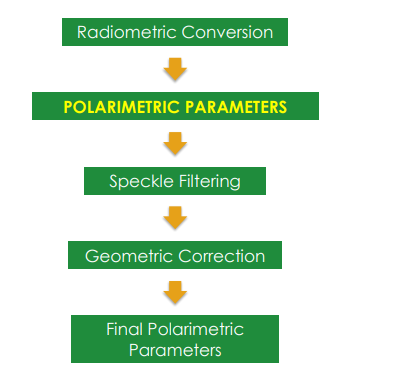
\includegraphics[width=0.4\textwidth]{figures/snap.PNG}
    \decoRule
    \caption[Generating Polarimetric Parameters in SNAP]{Generating Polarimetric Parameters in SNAP.}
    \label{fig:undercatch}
\end{figure}

	
	%\begin{wrapfigure}{l}{0.25\textwidth}
%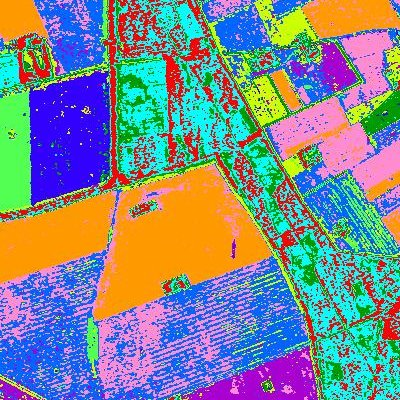
\includegraphics[width=0.9\linewidth]{figures/PolSAR.jpg}
%\caption{Ttulo 1}
%\label{F:figuranotexto}
%\end{wrapfigure}


\subsection*{Example math equations}
%-----------------------------------------------------------
%\begin{align*}
%L(\alpha,  \lambda|  \bm{x})&=\prod_{i=1}^n{f(x_i|\alpha, \lambda )}\\
                                 %&= \prod_{i=1}^n\left[\frac{\lambda^{\alpha}}{\Gamma(\alpha)}\,x_i^{\alpha-1}\exp\left\{-\lambda x_i\right\}\right]\\
%&=\left(\frac{\lambda^{\alpha}}{\Gamma(\alpha)}\right)^n\prod_{i=1}^nx_i^{\alpha-1}\times \exp\left\{-\left(\lambda\sum_{i=1}^n x_i \right)\right\}
%\end{align*}
%%----------------------------------------------------------
\begin{align}
\label{eq:em}
\ell(\alpha, \lambda| \bm{x}) &=\log\left[\left(\frac{\lambda^{\alpha}}{\Gamma(\alpha)}\right)^n\prod_{i=1}^nx_i^{\alpha-1}\times \exp\left\{-\left(\lambda\sum_{i=1}^n x_i \right)\right\}\right]\nonumber\\
&=\log\left(\frac{\lambda^{\alpha}}{\Gamma(\alpha)}\right)^n+\log\left[\prod_{i=1}^nx_i^{\alpha-1}\right]-\lambda\sum_{i=1}^nx_i\nonumber\\
&=n\log\left(\frac{\lambda^{\alpha}}{\Gamma(\alpha)}\right)+(\alpha-1)\log\prod_{i=1}^nx_i-\lambda\sum_{i=1}^nx_i\nonumber\\
&=n\log(\lambda^{\alpha})-n\log(\Gamma(\alpha))+(\alpha-1)\sum_{i=1}^n\log(x_i)-\lambda\sum_{i=1}^nx_i\nonumber\\
&=n\alpha\log \lambda -n\log(\Gamma(\alpha)) +(\alpha-1)\sum_{i=1}^n\log(x_i)-\lambda\sum_{i=1}^nx_i.
	\end{align}
%----------------------------------------------------------
\begin{figure}
    \centering
    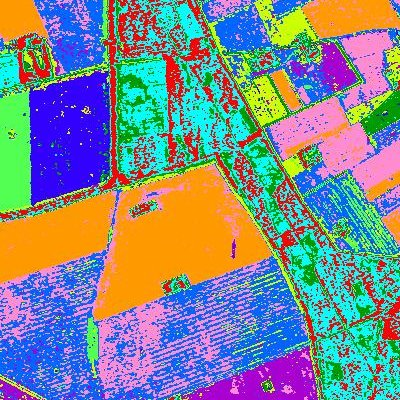
\includegraphics[width=0.5\textwidth]{figures/PolSAR.jpg}
    \decoRule
    \caption[Example plot]{Example plot.}
    \label{fig:undercatch}
\end{figure}

%-------------------------------------------------------

%\begin{table}[h]
%\centering
%\caption{\label{tab1}Comparação de tempos. }
%\begin{tabular}{l c c }
%\toprule[1pt] \textbf{Amostra (N)} \ \ \  \ \ \  & \textbf{Tempo de Execução (C)}\ \ \ \ \ \ \  &\textbf{Tempo de Execução (Ox)} \\\midrule[0.5pt]
%$20$ & 7.6810 s  &  5.01 s \\
%$30$ & 9.6260 s     & 5.34 s \\
%$50$ &  10.0310 s & 5.99 s \\
%$100$ & 15.5420 s & 8.07 s \\
%$200$ & 20.5860 s & 9.64 s \\
%$500$ & 29.0890  s & 15.12 s \\
%\bottomrule[1pt]
%\end{tabular}
%\caption[Precipitation datasets]{List of datasets used in the analysis of daily precipitation uncertainty carried over i}\label{tab:1}
%\end{table}
%------------------------------------------------------


%\begin{table}[]
%\centering
%\begin{tabular}{@{}llll@{}}
%\toprule
%Dataset name & Period & Spatial res. & Data source \\ \midrule
%E-OBS        & 2000--2016 & \ang{0.25}                            & Station data \\
%EURO4M-APGD  & 2000--2008 & \SI{5}{\kilo\metre}                   & Station data \\
%HMR          & 2000--2013 & \SI{5.5}{\kilo\metre}                 & Reanalysis \\
%ARCIS        & 2000--2015 & \textasciitilde{} \SI{5}{\kilo\metre} & Station data \\
%CHIRPS       & 2000--2016 & \ang{0.05}                            & Station data + satellite \\
%CPC          & 2000--2016 & \ang{0.5}                             & Station data \\
%CMORPH       & 2000--2016 & \ang{0.25}                            & Satellite \\
%PERSIANN-CDR & 2000--2016 & \ang{0.25}                            & Satellite \\ \bottomrule
%\end{tabular}
%\caption[ Italy]{List of datasets used in the analysis of daily precipitation uncertainty  references.}\label{tab:2}
%\end{table}




 
%\chapter{Data}\label{chp:itaobs}

\chapter{Methodology} \label{chp:models}

As introduced in Chapter ~\ref{chp:int}, several methods have also been proposed to...\\
This Chapter is organized as follows.


\chapter{Results}\label{chp:results}
This chapter will discuss the results obtained during the development of this project.\\
As described in the previous chapter... 
\chapter{Conclusions and future perspectives}\label{chp:conclusions}

As part of the project, we...\\

The work presented in this thesis..\\

Despite these limitations, we believe that the approach ...\\

In conclusion, ....

%\include{todo}

%%
%% Parte pós-textual
%%
\backmatter

% Apêndices
% Comente se não houver apêndices
\newpage


%\appendix

%------------------------------------------------------------
%activar luego
    %\refstepcounter{chapter}
    %\chapter*{\appendixname\enskip\thechapter}
    %\addcontentsline{toc}{chapter}{\appendixname\enskip\thechapter}
    %
    %\section{Section in Appendix A}
	%
		
%
    \refstepcounter{chapter}
    %\chapter*{\appendixname\enskip\thechapter}
    %\addcontentsline{toc}{chapter}{\appendixname\enskip\thechapter}

    %\section{ Appendix A}
			%\chapter{Software and programs used in this thesis}  \label{appendix_software}
This PhD project required a vast amount of computing, preprocessing, analysis and plotting.
None of this would have been possible without the large number of different software packages used, all of which are free to use, and most of which are open source.
The following is a non-comprehensive list of the software used:
\begin{multicols}{2}
    \begin{description}
        \item[R] \citet{R}
        \item[CDO] \citet{CDO}
        \item[NCO] \citet{Zender2008}
        \item[Python] \citet{python}
        \item[netCDF] \citet{netcdf}
        \item[ScyPy] \citet{Jones2007}
        \item[GDAL] \citet{GDAL}
    \end{description}
\end{multicols}

Most of the data analysis and plotting was carried out using R. Several R packages were extremely useful and deserve a special mention:
\begin{multicols}{2}
    \begin{description}
 \item[ncdf4] \citet{ncdf4}
 \item[ggplot2] \citet{ggplot2}
 \item[patchwork] \citet{patchwork}
 \item[ggspatial] \citet{ggspatial}
% \item[ggalt] \citet{ggalt}
 \item[ggrepel] \citet{ggrepel}
 \item[RColorBrewer] \citet{RColorBrewer}
% \item[shinyjs] \citet{shinyjs}
% \item[shinydashboard] \citet{shinydashboard}
 \item[sf] \citet{sf}
 \item[stars] \citet{stars}
 \item[raster] \citet{raster}
 \item[rnaturalearth] \citet{rnaturalearth}
 \item[mapedit] \citet{mapedit}
 \item[leaflet] \citet{leaflet}
 \item[shiny] \citet{shiny}
 \item[dplyr] \citet{dplyr}
 \item[tidyr] \citet{tidyr}
 \item[glue] \citet{glue}
 \item[readr] \citet{readr}
 \item[profvis] \citet{profvis}
 \item[purrr] \citet{purrr}
 \item[furrr] \citet{furrr}
 \item[future] \citet{future}
 \item[futile.logger] \citet{futile.logger}
 \item[optparse] \citet{optparse}
 \item[lubridate] \citet{lubridate}
    \end{description}
\end{multicols}

This thesis was typeset in \LaTeX.

		%----------------------------------------
\cleardoublepage
%\newpage
% \phantomsection
%------------------------------------
%	ABBREVIATIONS
%------------------------------------

%\begin{abbreviations}{ll} % Include a list of abbreviations (a table of two columns)

\textbf{SAR} & Synthetic Aperture Radar\\
\textbf{UAVSAR} & Uninhabited Aerial Vehicle Synthetic Aperture Radar\\
\textbf{PDF} & Probability density function\\
\textbf{CDF} & Cumulative distribution function\\
\textbf{ASF} & Alaska Satellite Facility\\
\textbf{ESA} & Agencia Espacial Europea\\
\textbf{ASF} & Alaska Satellite Facility\\
\textbf{ENL} & Equivalent Number of Looks\\
\textbf{SNAP} & Sentinel Application Platform\\
\textbf{ROI} & Region of Interest\\ 
\textbf{ROC} & Receiver Operating Characteristic \\
\textbf{AUC} & Area Under the ROC Curve
\end{abbreviations}


%------------------------------------
{
  \hypersetup{linkcolor=black}% para colocar color negro en la tabla de listas y figuras
  

\newpage
\addcontentsline{toc}{chapter}{\listfigurename}
\listoffigures
\cleardoublepage
\newpage
\addcontentsline{toc}{chapter}{\listtablename}
\listoftables

}
% É aconselhável criar cada apêndice em um arquivo à parte, digamos
% "apendice1.tex", "apendice.tex", ... "apendiceM.tex" e depois
% incluí-los com:
% \include{apendice1}
% \include{apendice2}
% ...
% \include{apendiceM}
\newpage
\cleardoublepage
%------------------------------------
%	BIBLIOGRAPHY
%------------------------------------

%\bibliographystyle{IEEEtran}
%\bibliography{mendeley_v2}
%\nocite{*}
\printbibliography[heading=bibintoc]

%\setlength{\parskip}{3.0pt}
% Bibliografia
% É aconselhável utilizar o BibTeX a partir de um arquivo, digamos "biblio.bib".
% Para ajuda na criação do arquivo .bib e utilização do BibTeX, recorra ao
% BibTeXpress em www.cin.ufpe.br/~paguso/bibtexpress
%\nocite{*}
%\bibliographystyle{plain}
%\bibliography{biblio}

% Cólofon
% Descomente para incluir uma pequena nota com referência à UFPEThesis
%\colophon

%% Fim do documento
\end{document}
